\documentclass[11pt]{beamer}
\usepackage[utf8]{inputenc}
\usepackage[T1]{fontenc}
\usepackage{lmodern}
\usepackage[english]{babel}
\usepackage{subcaption}
\usepackage{amsmath}
\usepackage{amsfonts}
\usepackage{hyperref}
\usepackage{multirow}
\usepackage{fontawesome}
\usepackage{amssymb}
\usepackage{graphicx}
\graphicspath{{figures/}}
\usetheme{Hannover}
%\setbeamertemplate{footline}[frame number]

\AtBeginSection[]
{
	\begin{frame}
		\frametitle{Table of Contents}
		\tableofcontents[currentsection]
	\end{frame}
}


\begin{document} 
	\author{Ignacio Condés Menchén}
	\title{Embedded Solution for Person Identification and Tracking with a Robot}
	\subtitle{Master in Telecommunication Engineering}
	\logo{
\includegraphics[height=1.5cm]{Portada_Logo.png}}
	\institute{Escuela Politécnica Superior\\
		Universidad Carlos III de Madrid}
	\date{July 23, 2020}
	%\subject{}
%	\setbeamercovered{transparent}
%	\setbeamertemplate{navigation symbols}{}

% COVER 
\begin{frame}[plain]
	\maketitle
\end{frame}

% TOC
\begin{frame}
	\frametitle{Table of Contents}
	\tableofcontents
\end{frame}

% 1.- INTRODUCTION
\section{Introduction}
%% Motivation
\subsection{Motivation}
\begin{frame}[allowframebreaks]
	\frametitle{Motivation}
		\begin{columns}
			\column{0.6\textwidth}
			Strong evolution in computer vision research and development.\\
			\vspace{0.2cm}
			Notable spreading of \textit{deep learning} techniques on computer vision: CNNs (\textit{Convolutional Neural Networks}).\\
			\vspace{0.8cm}			
			Multiple applications:
			\begin{itemize}
				\item Autonomous driving
				\item Medical diagnosis
				\item Surveillance
			\end{itemize}
			\column{0.4\textwidth}
			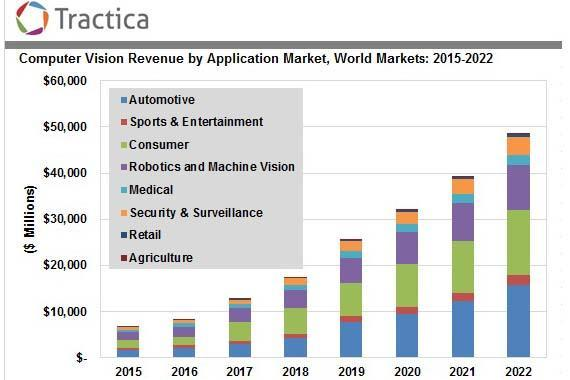
\includegraphics[width=0.9\linewidth]{cv_forecast_2022} \\
			\vspace{0.5cm}
			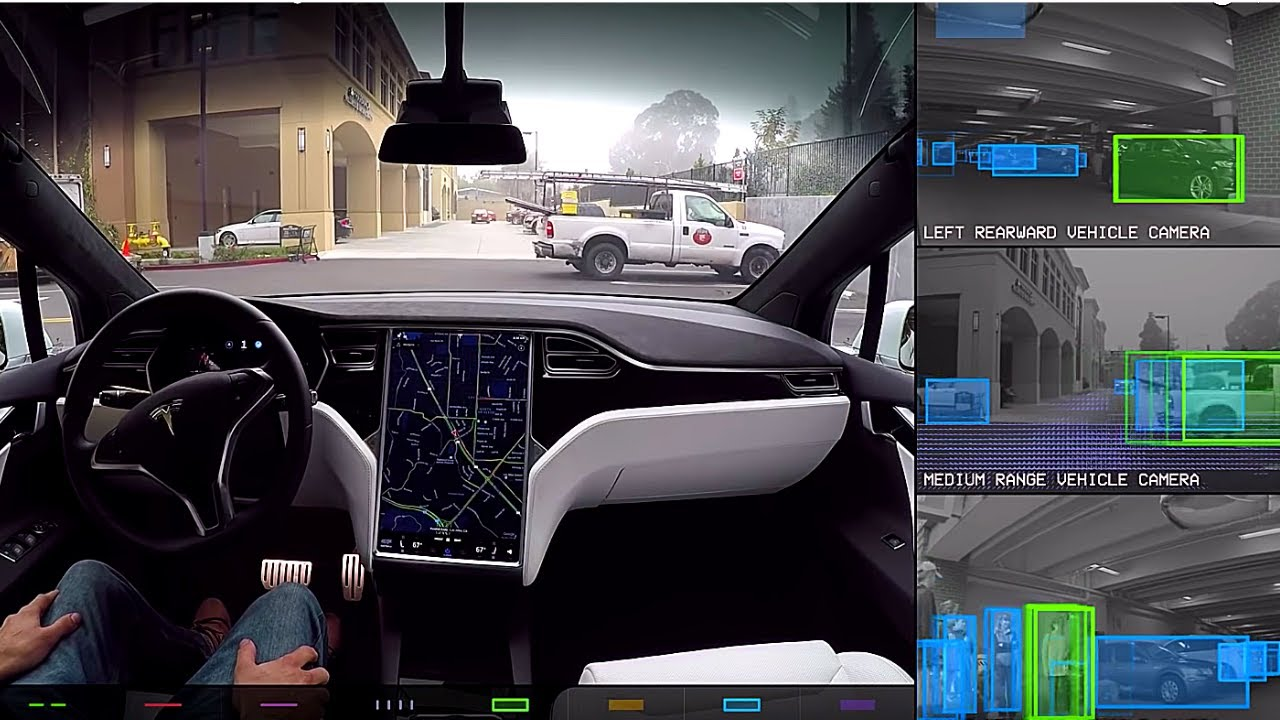
\includegraphics[width=0.9\linewidth]{tesla_autonomous_driving}
		\end{columns}
		\hfill
		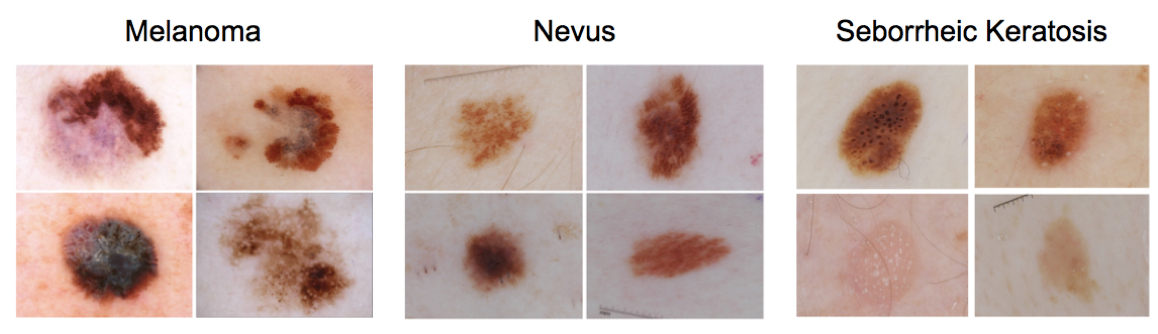
\includegraphics[width=0.75\linewidth]{ISIC}


		\begin{columns}
			\column{0.5\textwidth}
			Powerful applications in robotics as well:
			\begin{itemize}
				\item Remote inspections on hazardousness
				\item Precision surgery
				\item Social robotics
			\end{itemize}
			\column{0.5\textwidth}
			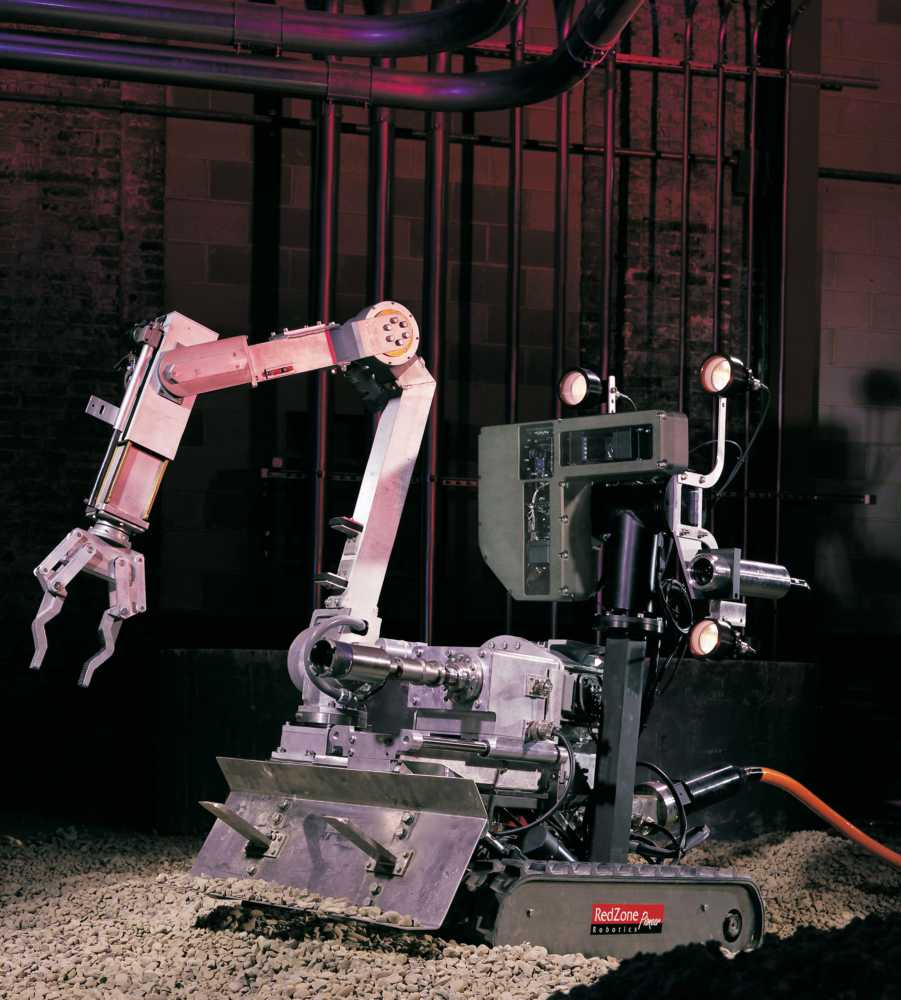
\includegraphics[width=0.5\linewidth]{pioneer_chernobyl} \\
			\vspace{0.5cm}
			\hfill
			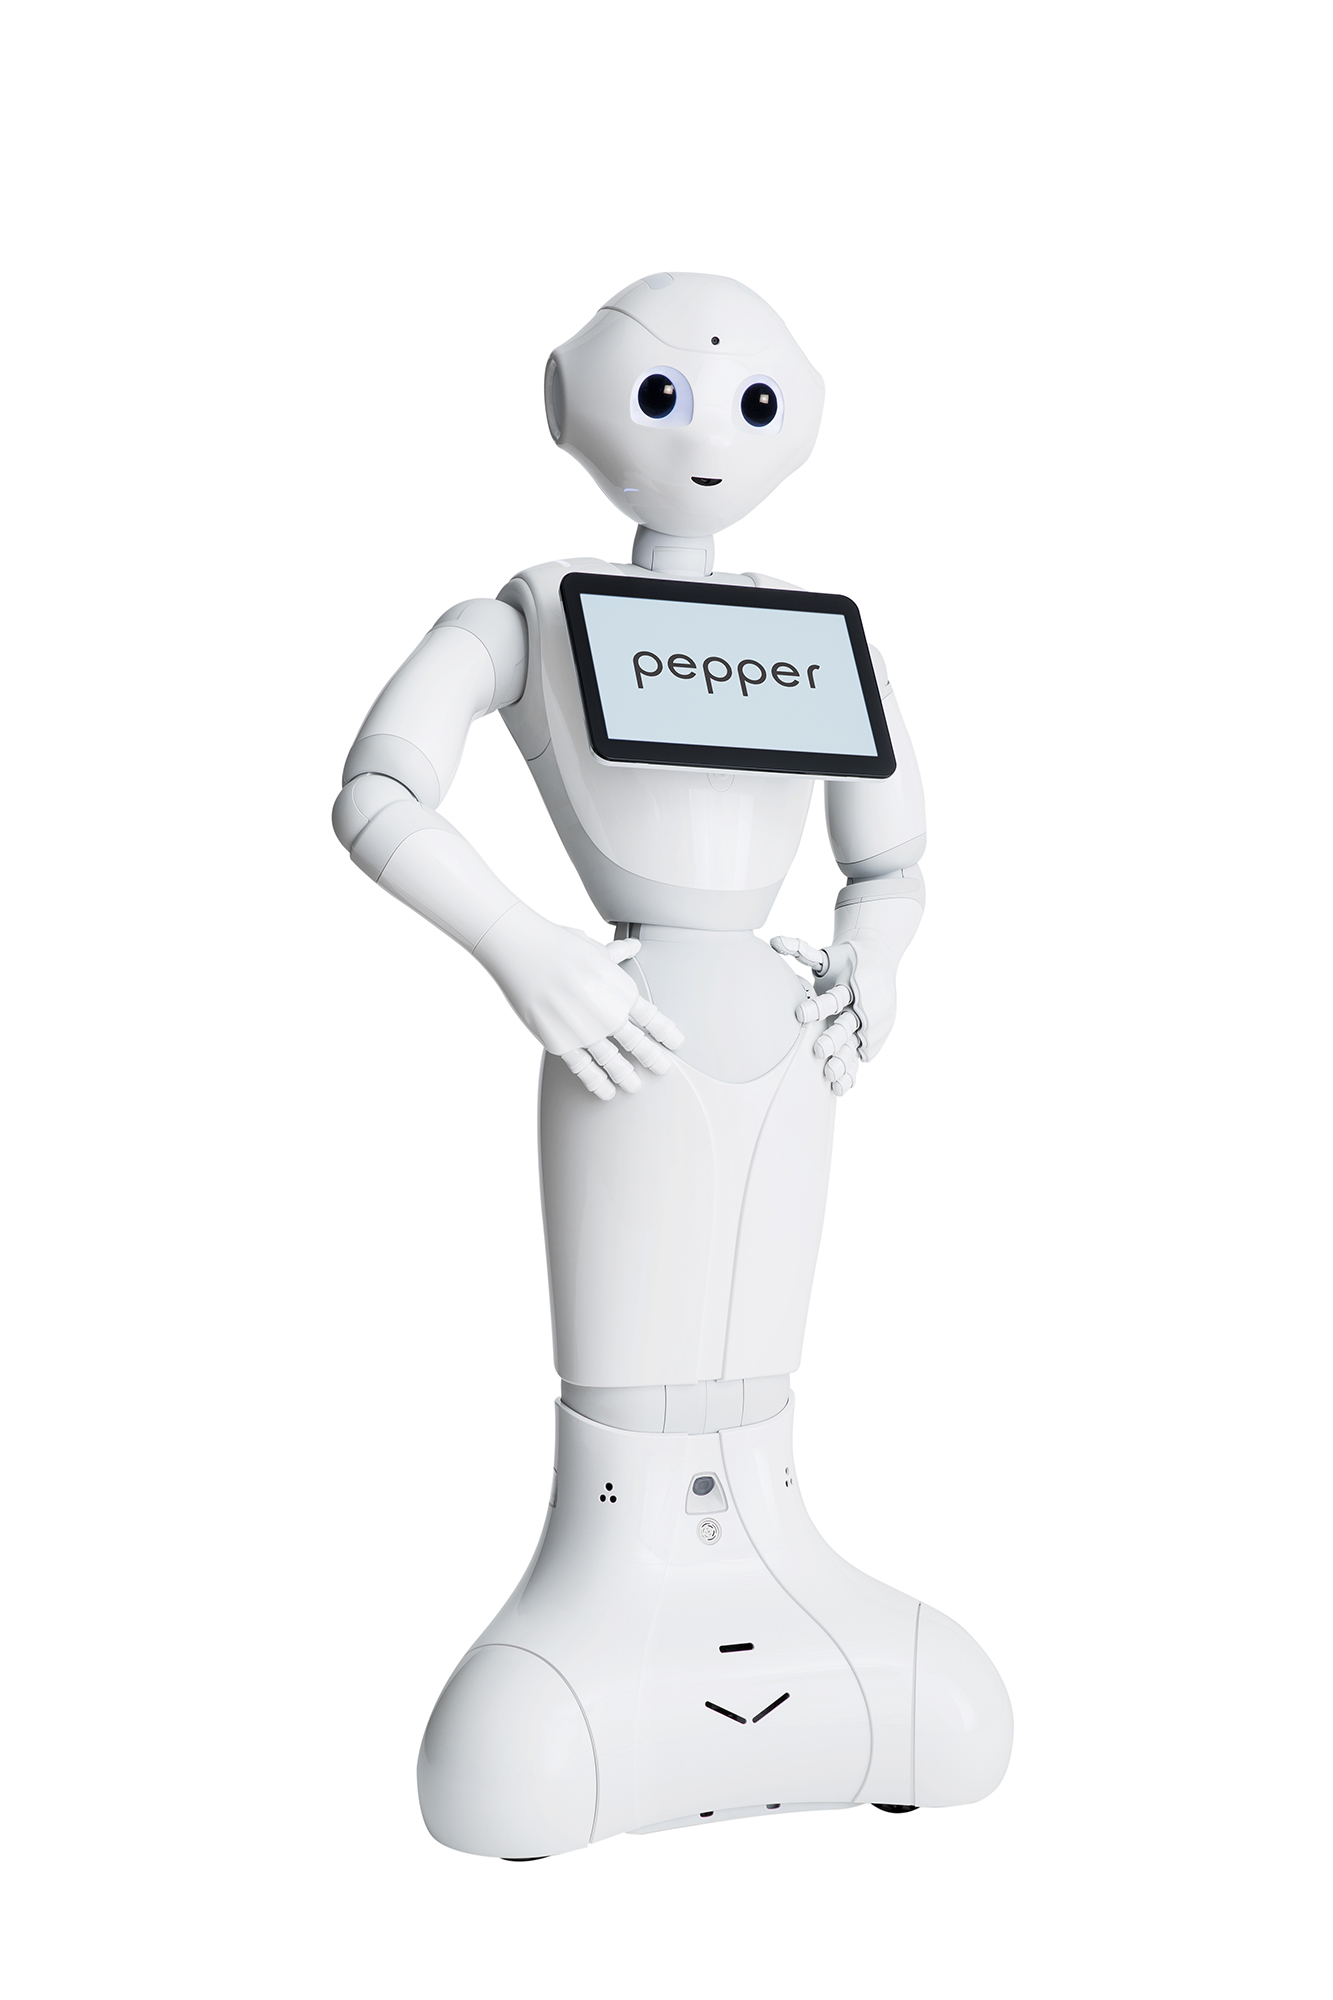
\includegraphics[width=0.5\linewidth]{pepper}
		\end{columns}
\end{frame}

%% Objectives
\subsection{Objectives}

\begin{frame}
	\frametitle{Objectives}
	Main goal: \alert{Autonomous robot that robustly follows a person.}\pause\\
	Subgoals:\\
	\vspace{0.2cm}
	\begin{itemize}
		\item Implement a real-time person following behavior on affordable hardware.
		\item Use only robust CNNs for the inference tasks.
		\item Enhance the robustness combining the CNNs with optical tracking.
	\end{itemize}
	\begin{columns}
		\column{0.45\linewidth}
			\begin{center}
				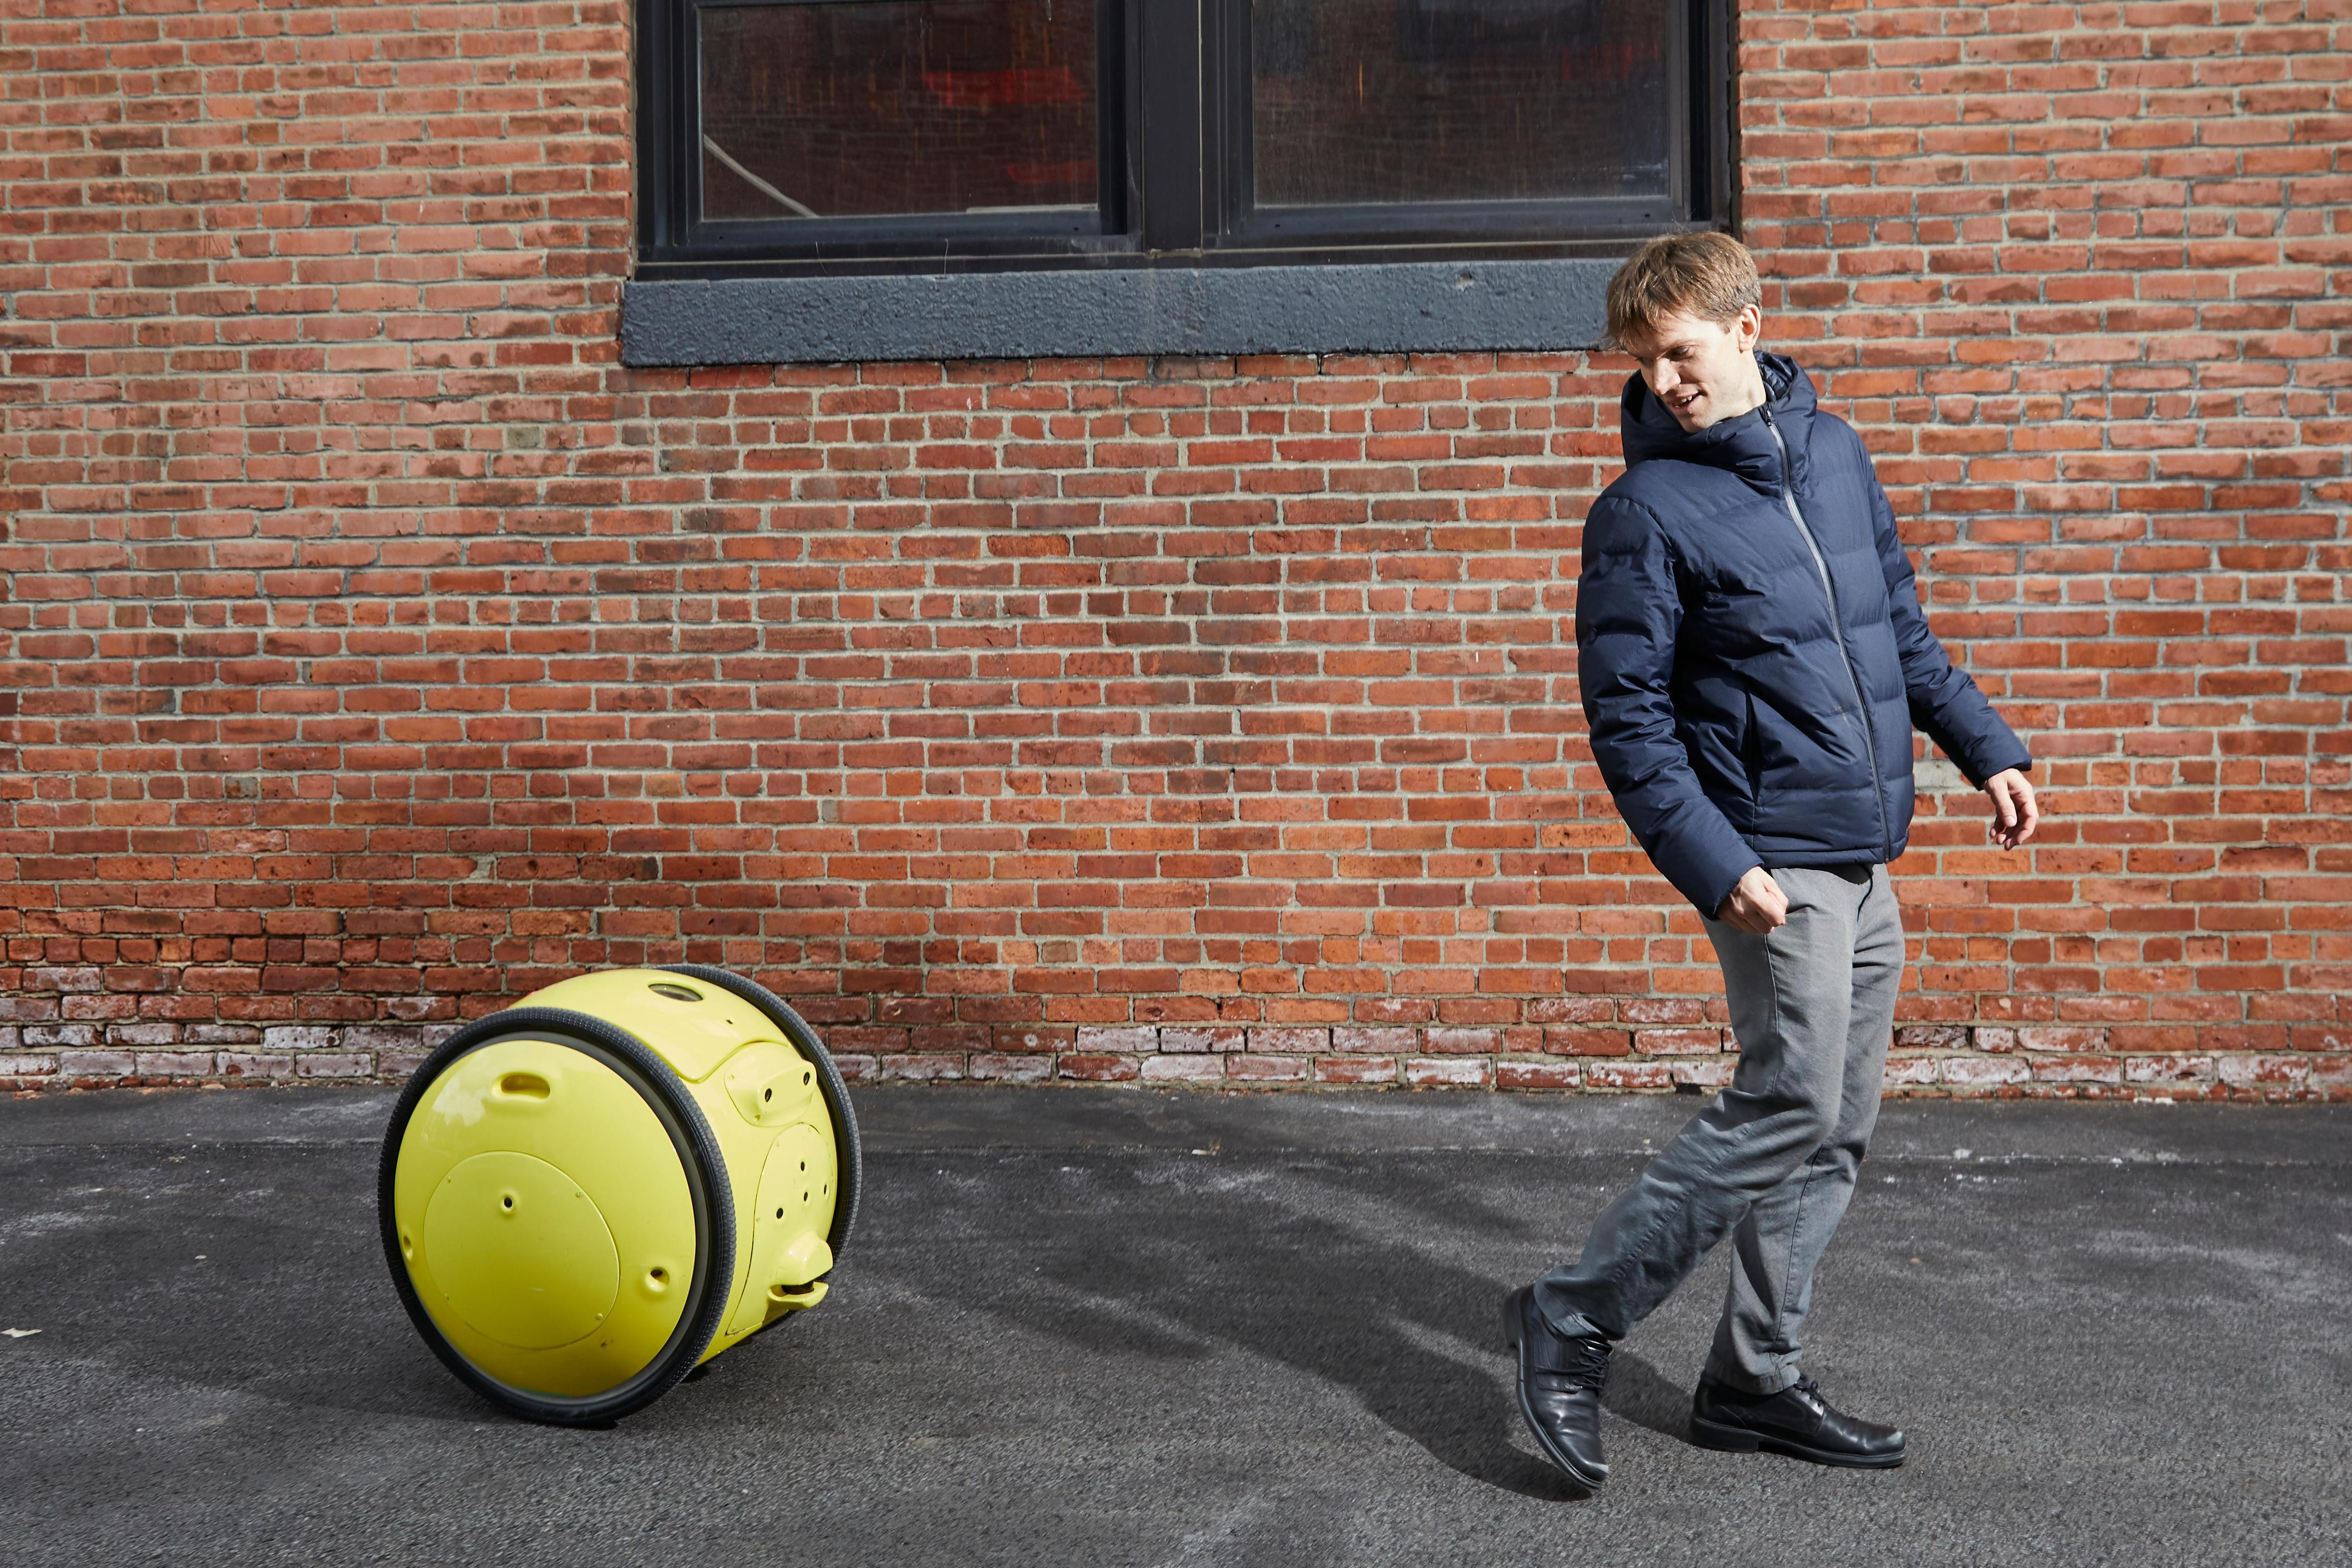
\includegraphics[width=0.9\linewidth]{robot_following} \\
			\end{center}
		\column{0.55\linewidth}
			\begin{center}
				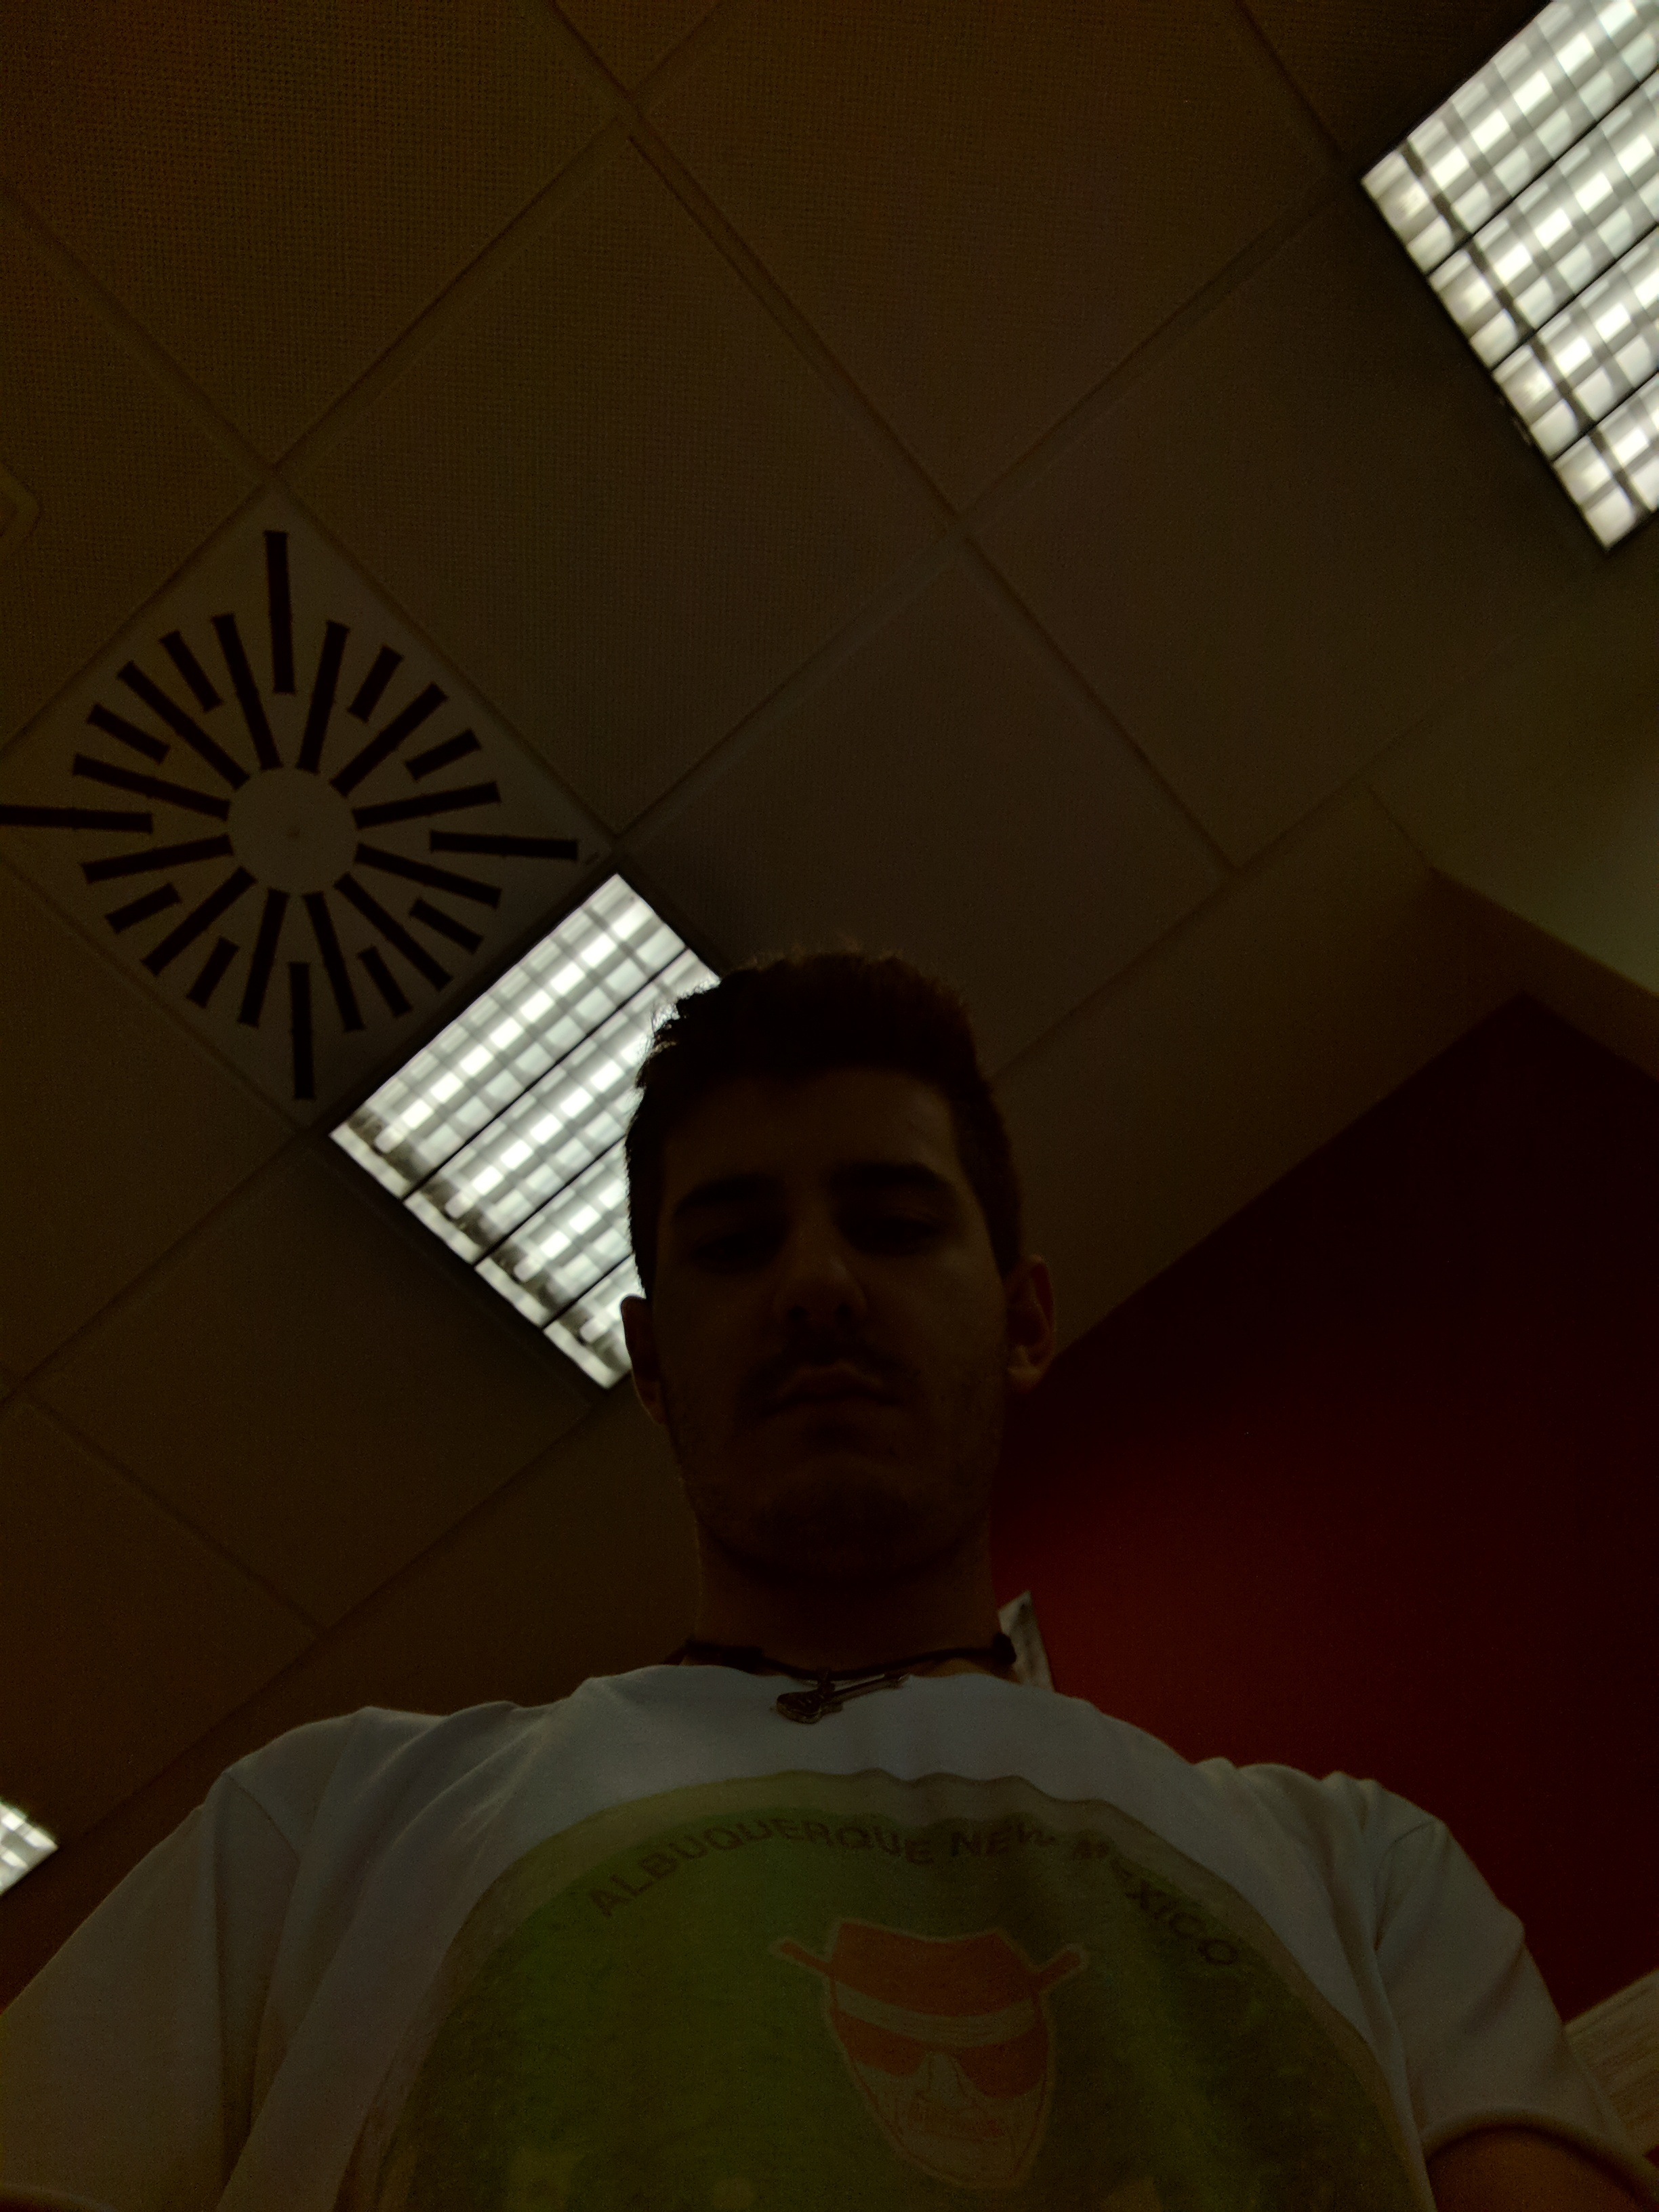
\includegraphics[width=0.36\linewidth]{light_ko}
				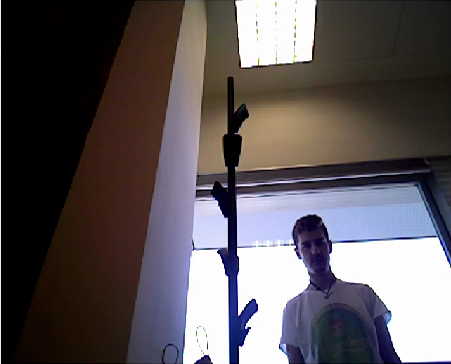
\includegraphics[width=0.6\linewidth]{light_ko_2} \\
			\end{center}
		
	\end{columns}
\end{frame}


% Proposed solution
\section{Proposed solution}
% Resources (HW + SW)
\subsection{Resources}
\begin{frame}
	\frametitle{Resources}
	\begin{columns}
		\column{0.5\textwidth}
		%		\vspace{-0.2cm}
		\textbf{Hardware}\\
		\vspace{0.55cm}
		\begin{center}
			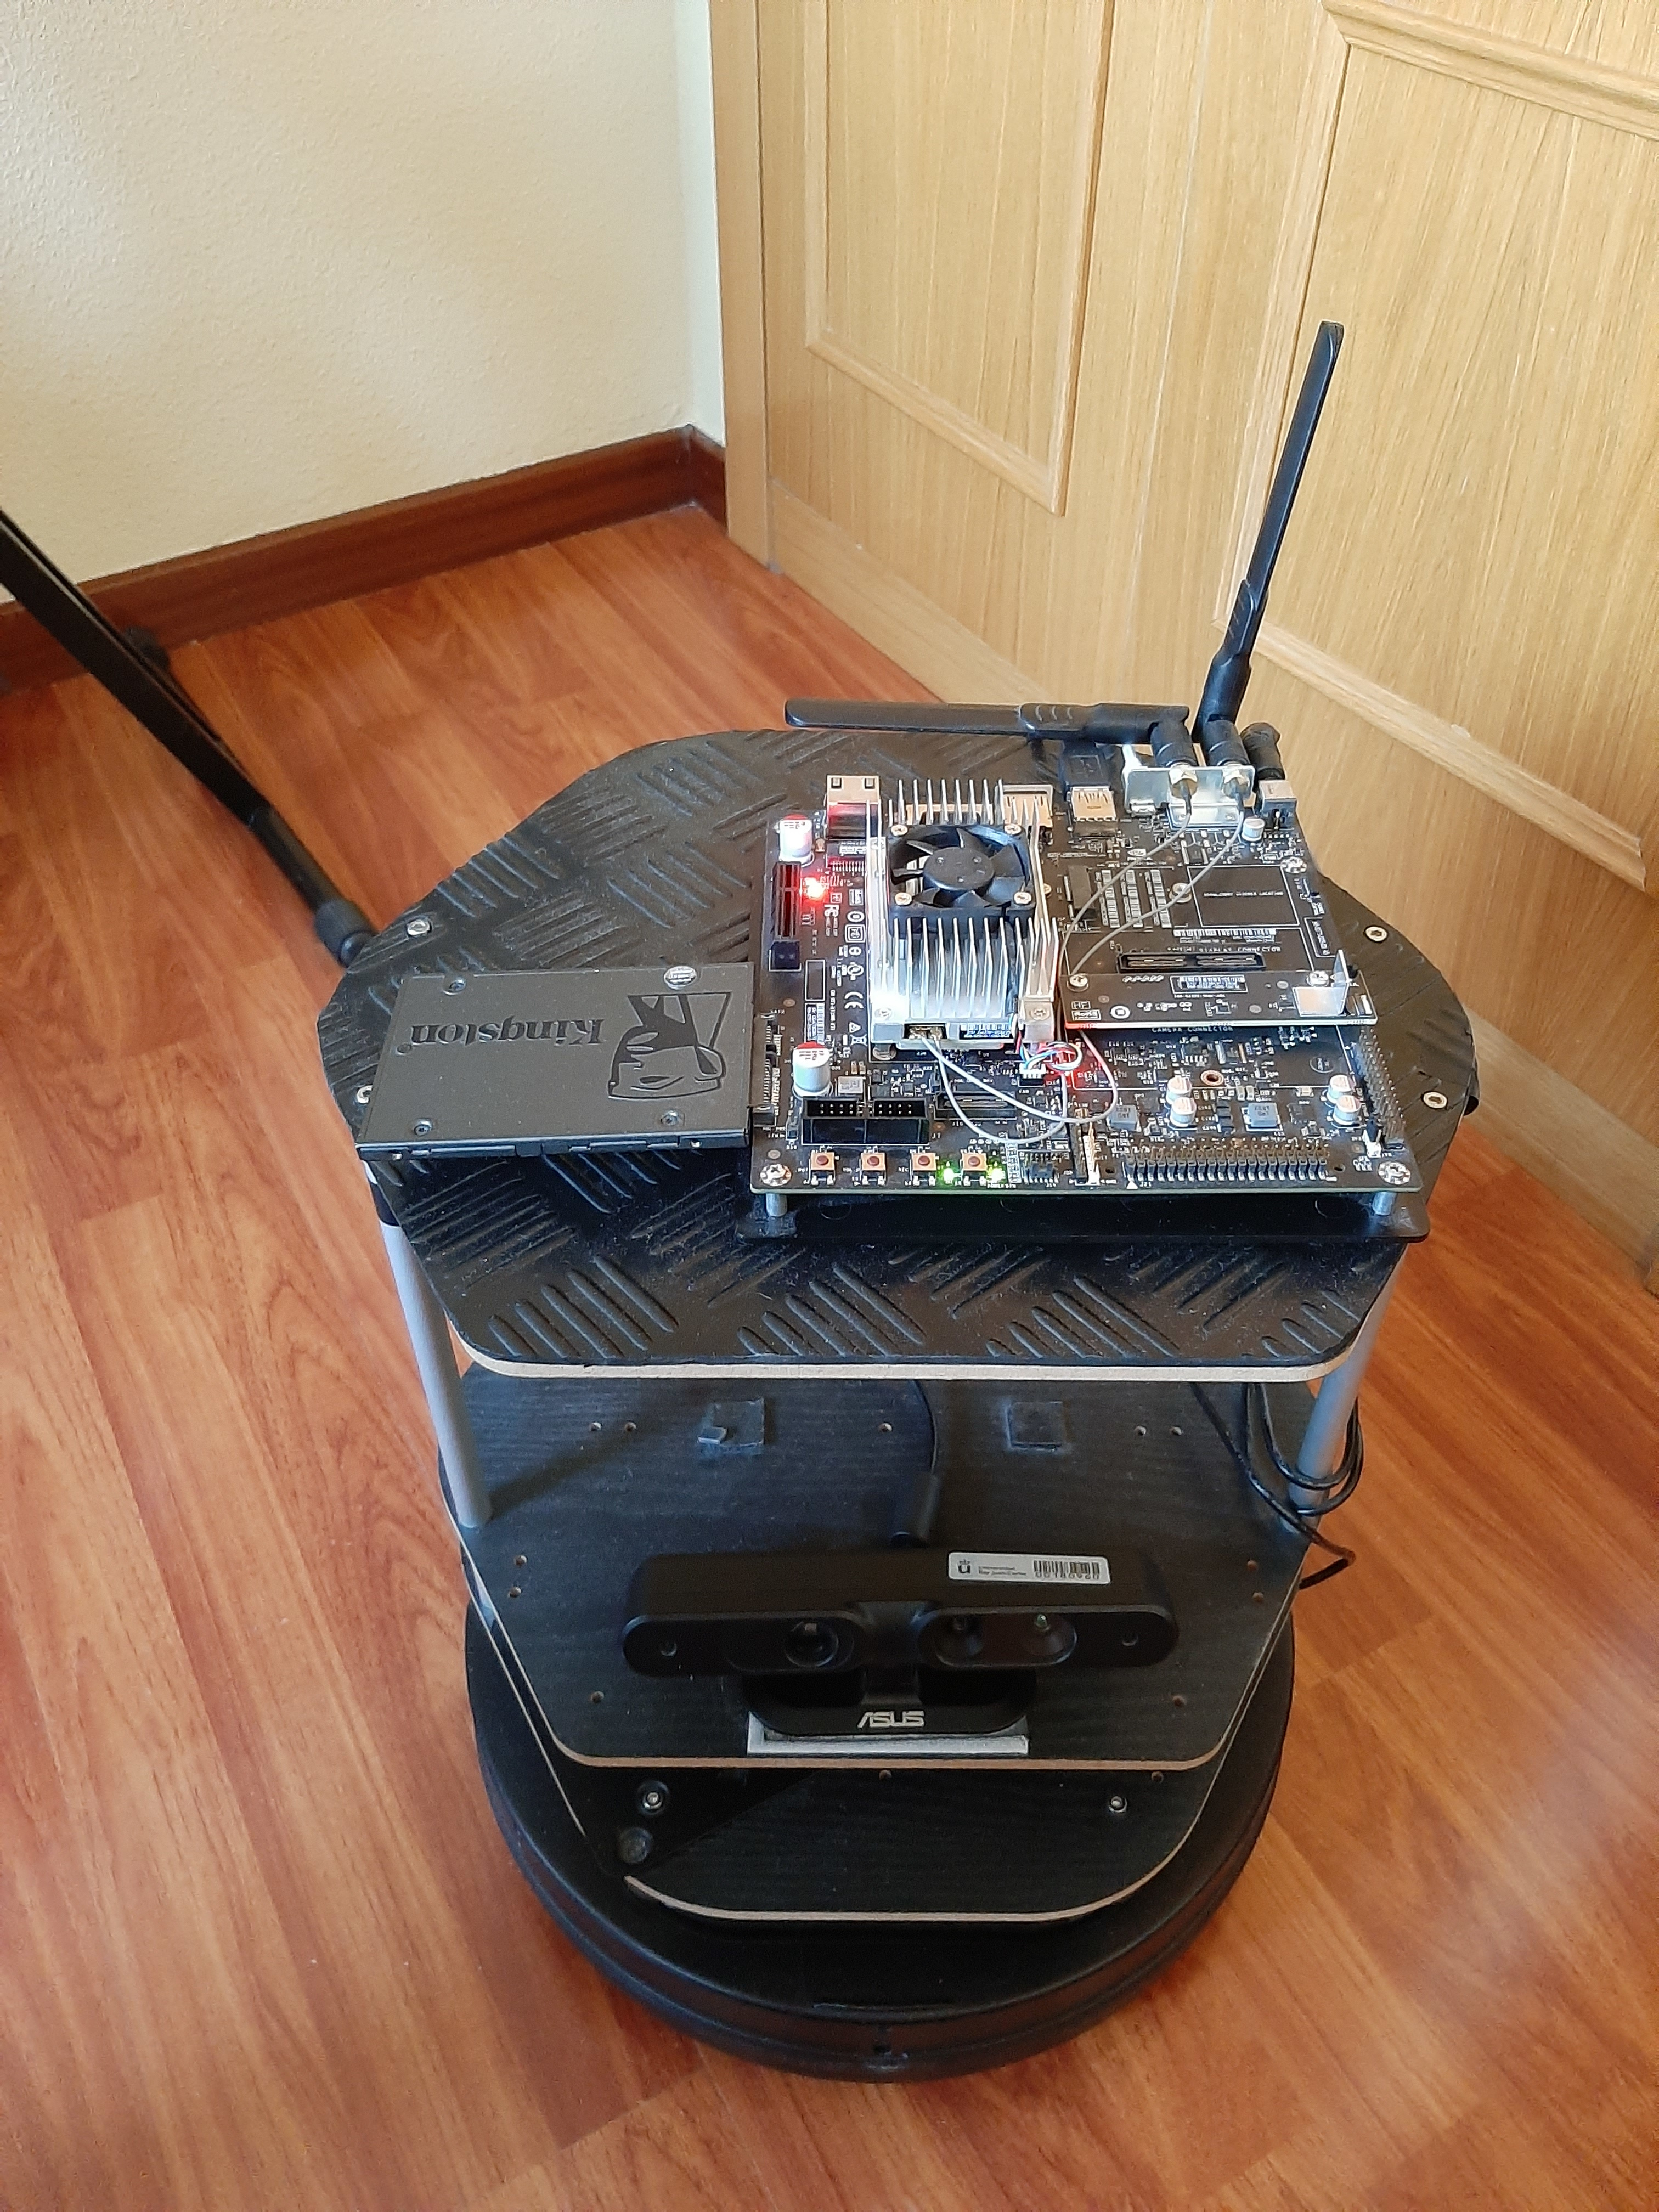
\includegraphics[width=0.6\linewidth]{setup_front} \\
		\end{center}
		\begin{itemize}
			\item NVIDIA Jetson TX2
%			\vspace{2cm}
			\item Turtlebot2
%			\vspace{1cm}
			\item ASUS Xtion Pro Live
		\end{itemize}
		
		\column{0.5\textwidth}
			\textbf{Software}\\
			\vspace{0.6cm}
			\begin{center}
				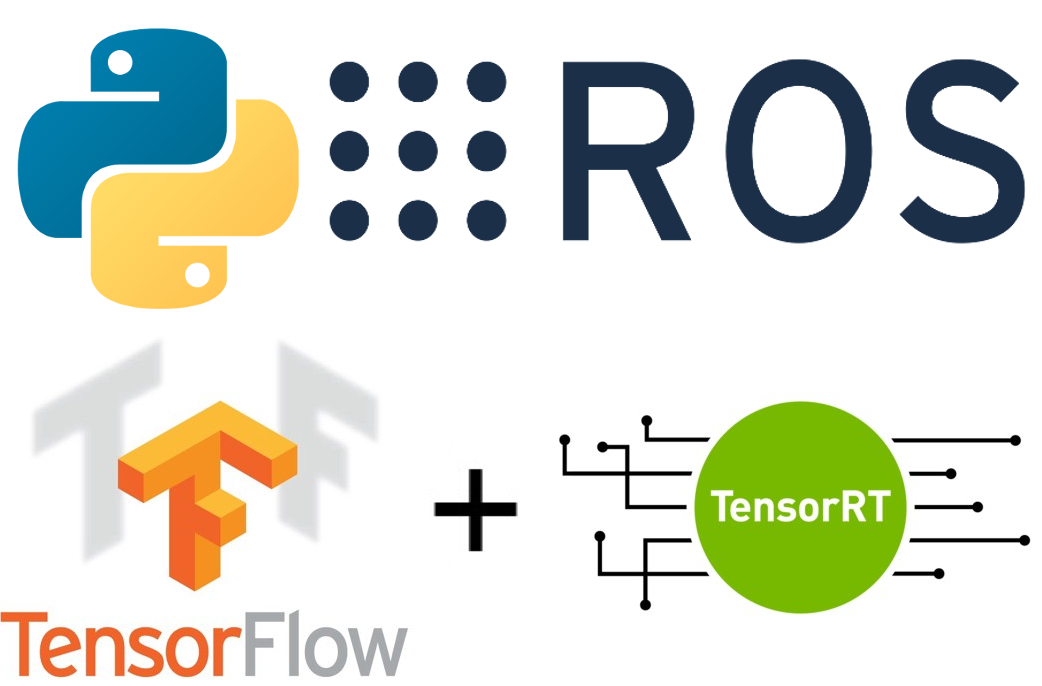
\includegraphics[width=0.9\linewidth]{software} \\
			\end{center}
			\vspace{0.4cm}
			\begin{itemize}
				\item Python 3.7
				\item ROS Melodic Morenia
				\item TensorFlow
				\item TensorRT
			\end{itemize}
	\end{columns}	
\end{frame}
\subsection{Design}
\begin{frame}
	\frametitle{Design}
	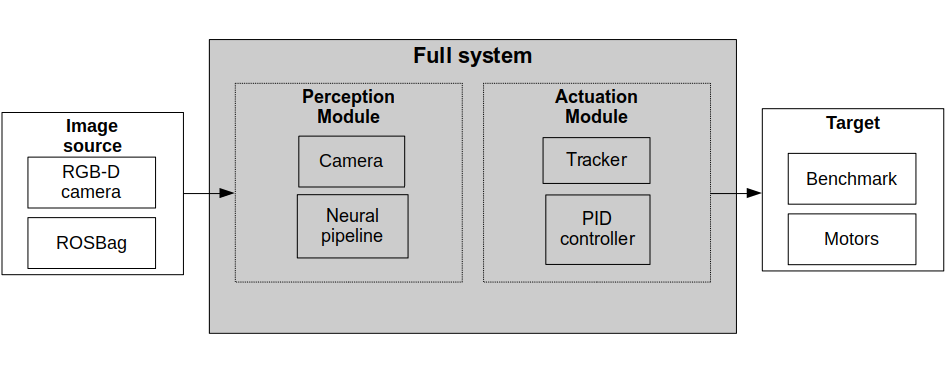
\includegraphics[width=\linewidth]{functional_architecture}
\end{frame}
\subsubsection{Perception Module}
\begin{frame}[allowframebreaks]
	\frametitle{Perception Module}
	Tasks to address:
	\begin{itemize}
%		\item Process external stimuli.
%		\item Based on deep learning: \alert{neural pipeline}.
		\item Person detection.
		\item Face detection.
		\item Face recognition.
	\end{itemize}
	\vspace{8cm}
	One devoted neural network for solving each task.\\
	\begin{columns}
		\column{0.5\textwidth}
		\begin{itemize}
			\item \textbf{Person detection:} object detection CNNs: YOLOv3, \alert{SSD}.
			\vspace{0.8cm}
			\item \textbf{Face detection:} specific face detection CNN: \alert{\texttt{faced}}.
			\vspace{0.8cm}
			\item \textbf{Face recognition:} face encoder to latent $\mathbb{R}^{128}$ space: \alert{FaceNet}.
		\end{itemize}
		\column{0.5\textwidth}
		\begin{center}
			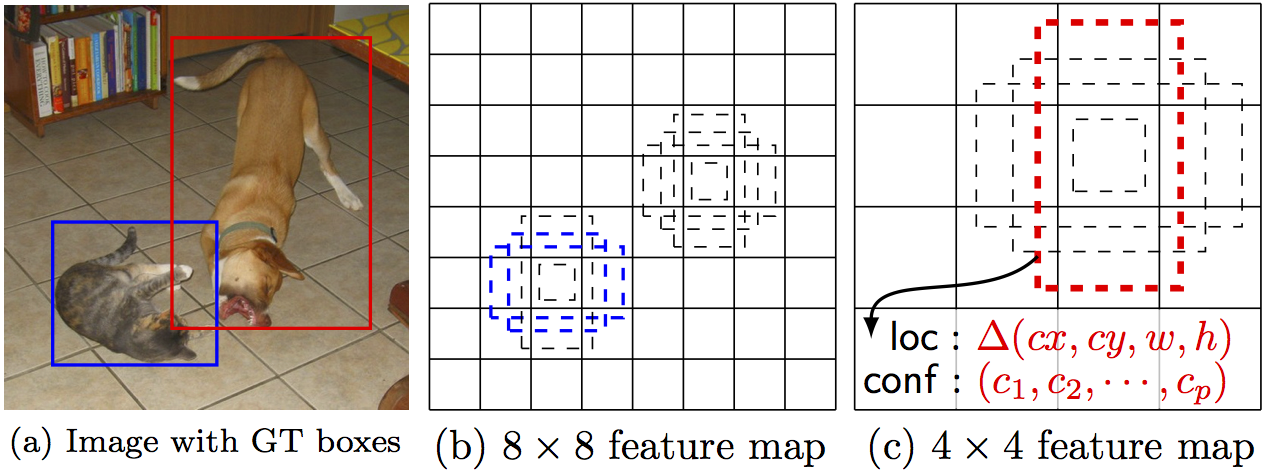
\includegraphics[width=\linewidth]{ssd_generated_boxes}\\
			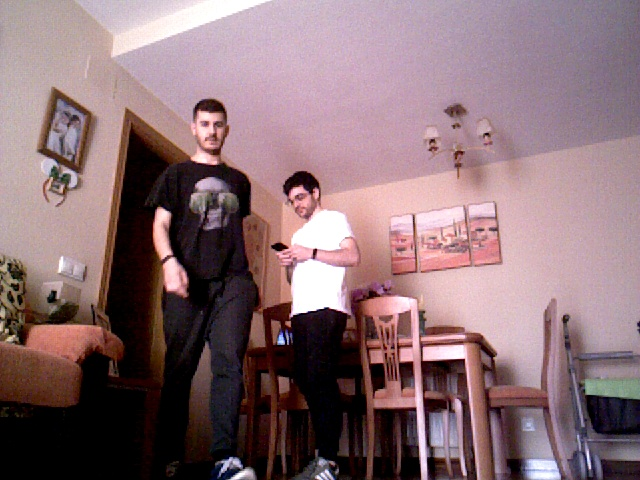
\includegraphics[width=0.4\linewidth]{face_detection}\\
			\vspace{0.5cm}
			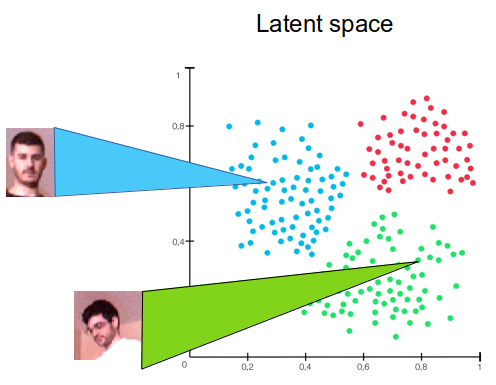
\includegraphics[width=0.6\linewidth]{face_encoder}\\
		\end{center}		
	\end{columns}
	\vspace{8cm}
	TensorRT used to optimize the networks across the neural pipeline.
	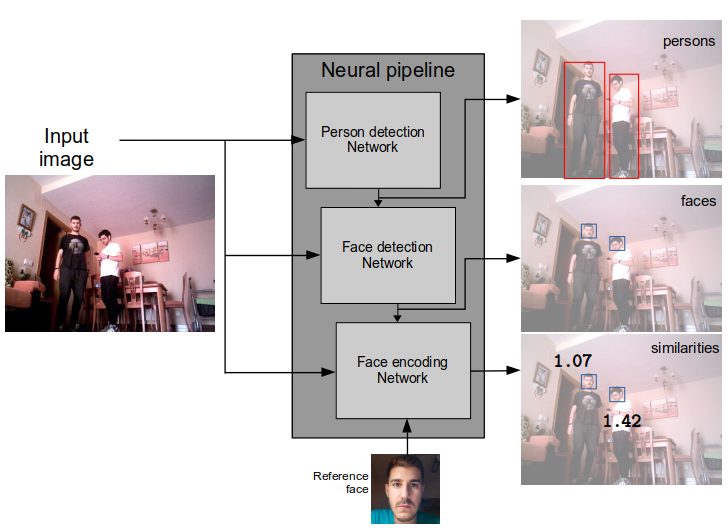
\includegraphics[width=0.9\linewidth]{neural_pipeline}
\end{frame}


\subsubsection{Actuation Module}
\begin{frame}[allowframebreaks]
	\frametitle{Actuation Module}
	Tasks to address:
	\begin{itemize}
		\item Track the persons.
		\item Move the robot.
	\end{itemize}
	\vspace{10cm}
	\begin{columns}
		\column{0.5\linewidth}
		Person tracker:
		\vspace{0.5cm}
		\begin{itemize}
			\item Based on optical flow estimation (Lucas-Kanade).
			\item Shift and transform the bounding box.
			\item \textit{Patience} for alleviating occlusions.
		\end{itemize}
		\column{0.5\linewidth}
			\begin{center}
				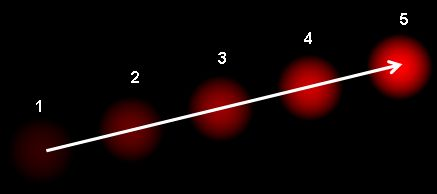
\includegraphics[width=0.6\linewidth]{optical_flow}
				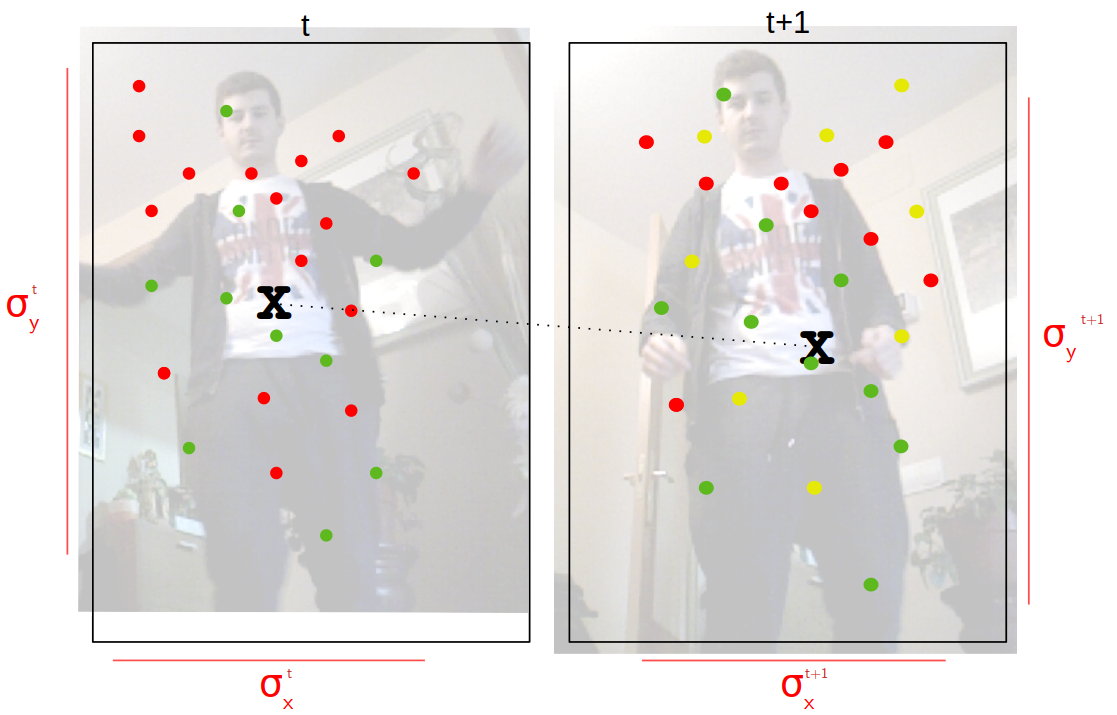
\includegraphics[width=\linewidth]{tracker_update}
			\end{center}
	\end{columns}
	\vspace{6cm}
	\begin{columns}
	\column{0.5\linewidth}
	PID Controllers:
	\vspace{0.5cm}
	\begin{itemize}
		\item Closed-loop control system.
		\item One per degree of freedom.
		\item Reactive responses.
		\item Safe zones for smooth response.
	\end{itemize}
	\column{0.5\linewidth}
	\begin{center}
		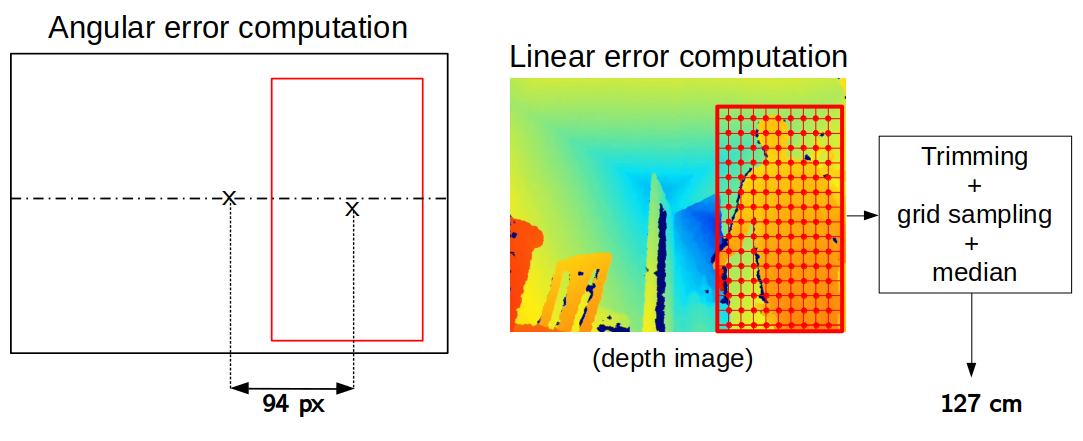
\includegraphics[width=\linewidth]{controller_error_computation}\\
		\vspace{0.5cm}
		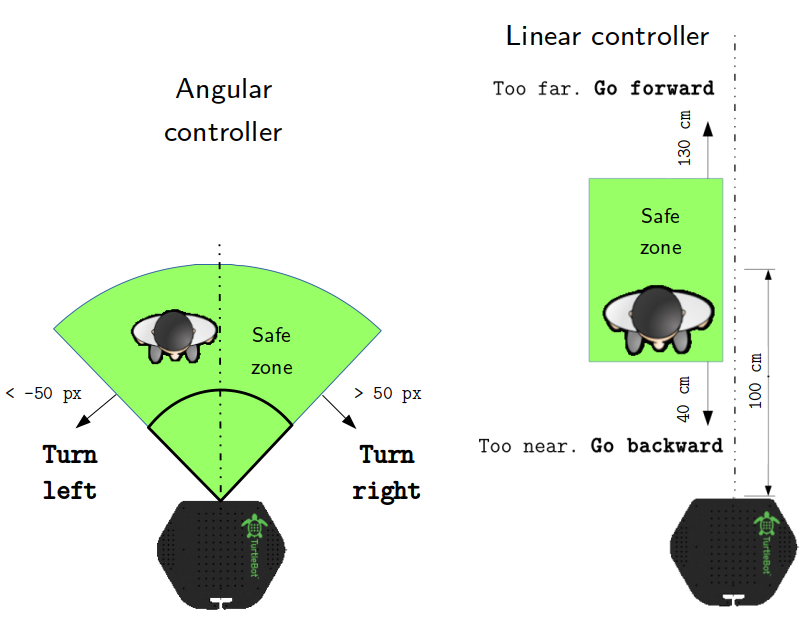
\includegraphics[width=\linewidth]{velocity_controllers}

	\end{center}
\end{columns}
	
\end{frame}

\begin{frame}
	\frametitle{Design summary}

	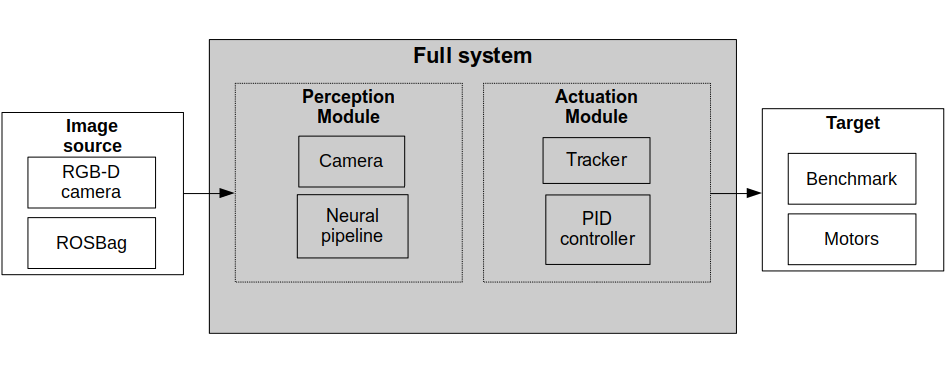
\includegraphics[width=\linewidth]{functional_architecture}
	
\end{frame}

\section{Results}
\begin{frame}
	\frametitle{Person detection}
	Precision and inference time: SSD vs. YOLOv3 tiny
	\begin{center}
		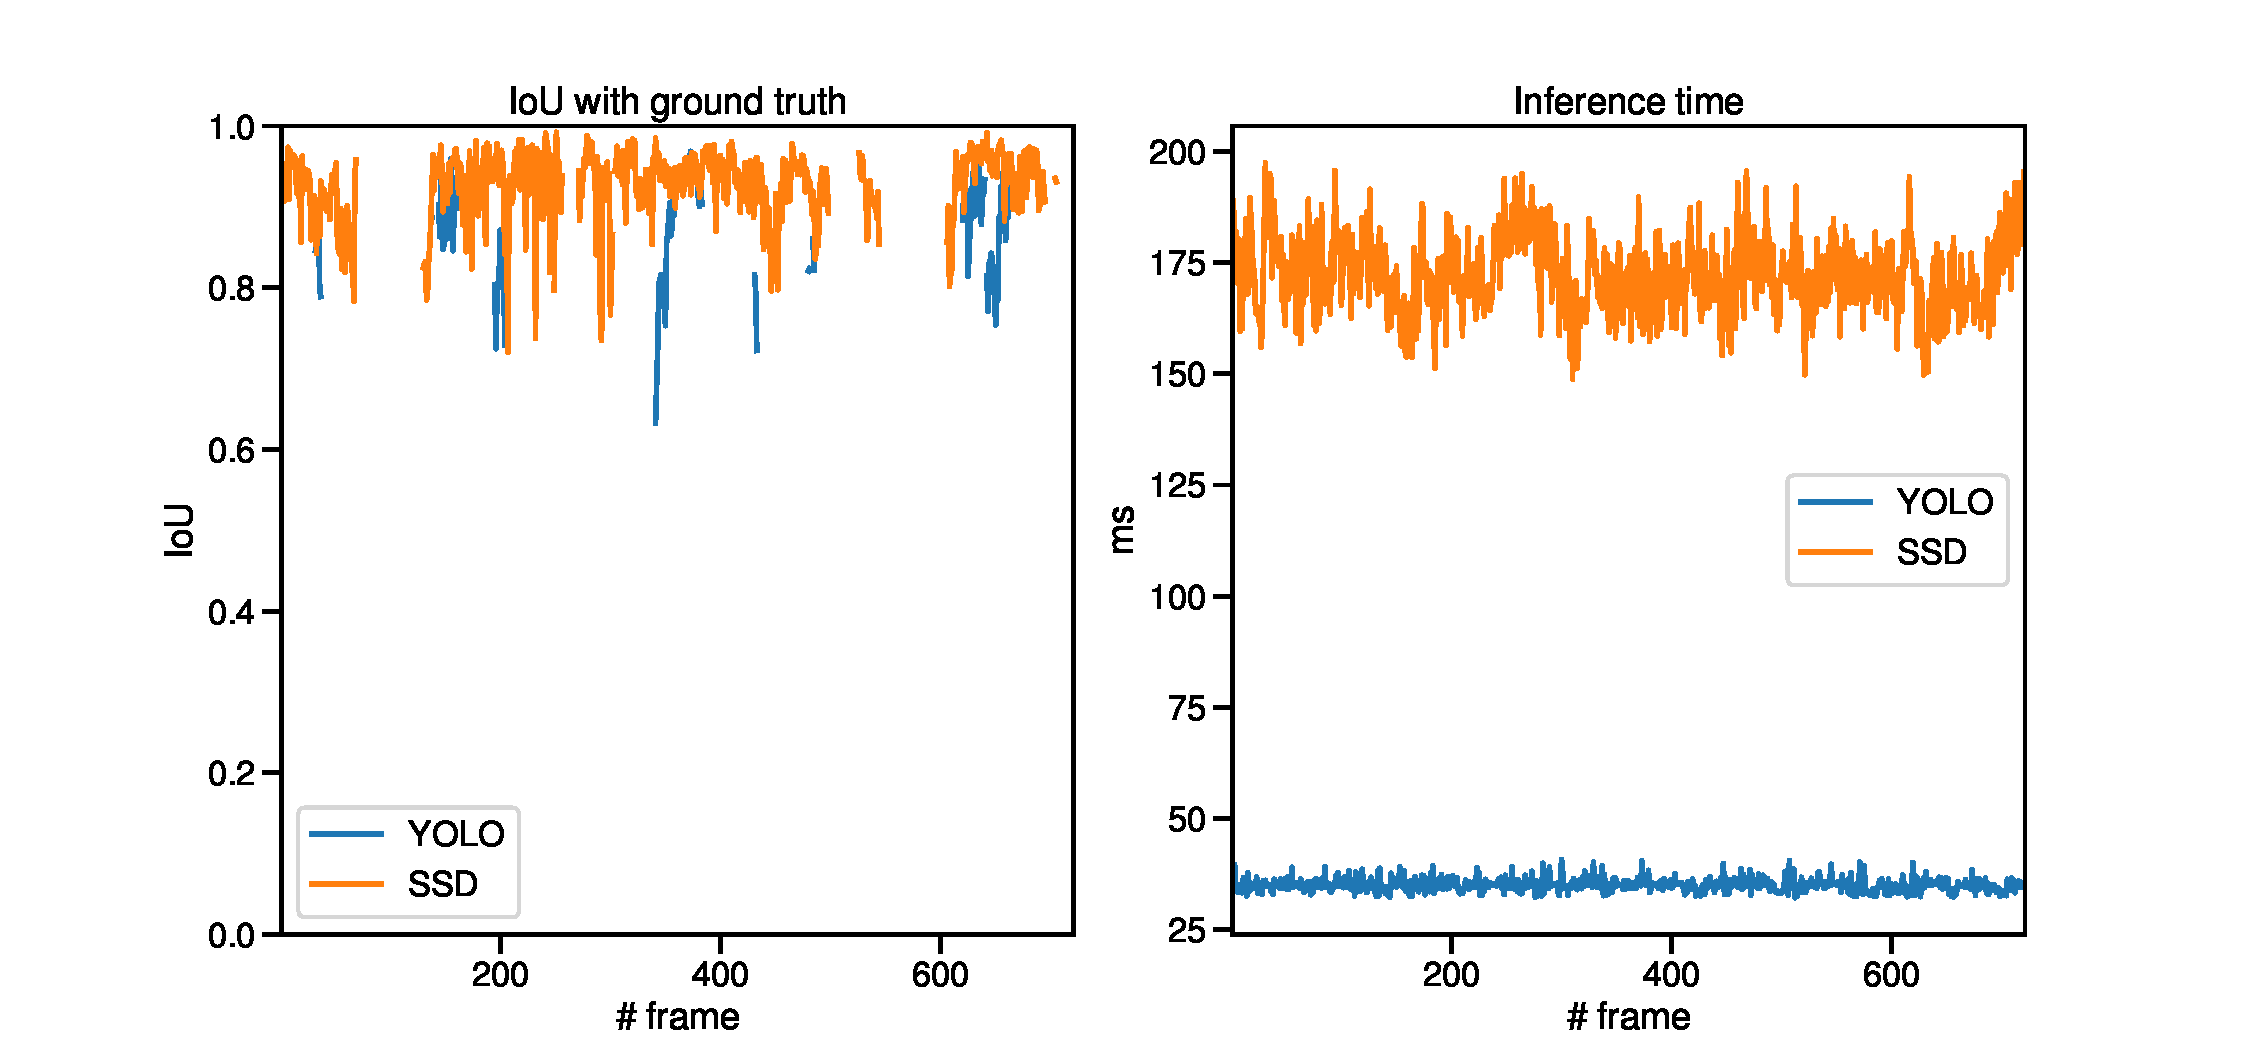
\includegraphics[width=0.8\linewidth]{test1}
	\end{center}
	
	\begin{table}[h]
		\tiny
		\begin{tabular}{|l|c|c|}
			\hline
			& \textbf{YOLO}             & \textbf{SSD}              \\ \hline
			\textbf{IoU}            & 0.858 $\pm$  0.068 & 0.926 $\pm$  0.044 \\ \hline
			\textbf{Inf. time (ms)} & 35.003 $\pm$ 1.503 & 172.237 $\pm$ 8.791 \\ \hline
			\textbf{Frames with detection} & 123 (17.06\%) & 533 (73.93\%) \\ \hline
		\end{tabular}
	\end{table}
	
\end{frame}

\begin{frame}
	\frametitle{Face detection}
	Precision: neural detector (\texttt{faced}) vs Haar-features classifier.
	\begin{center}
		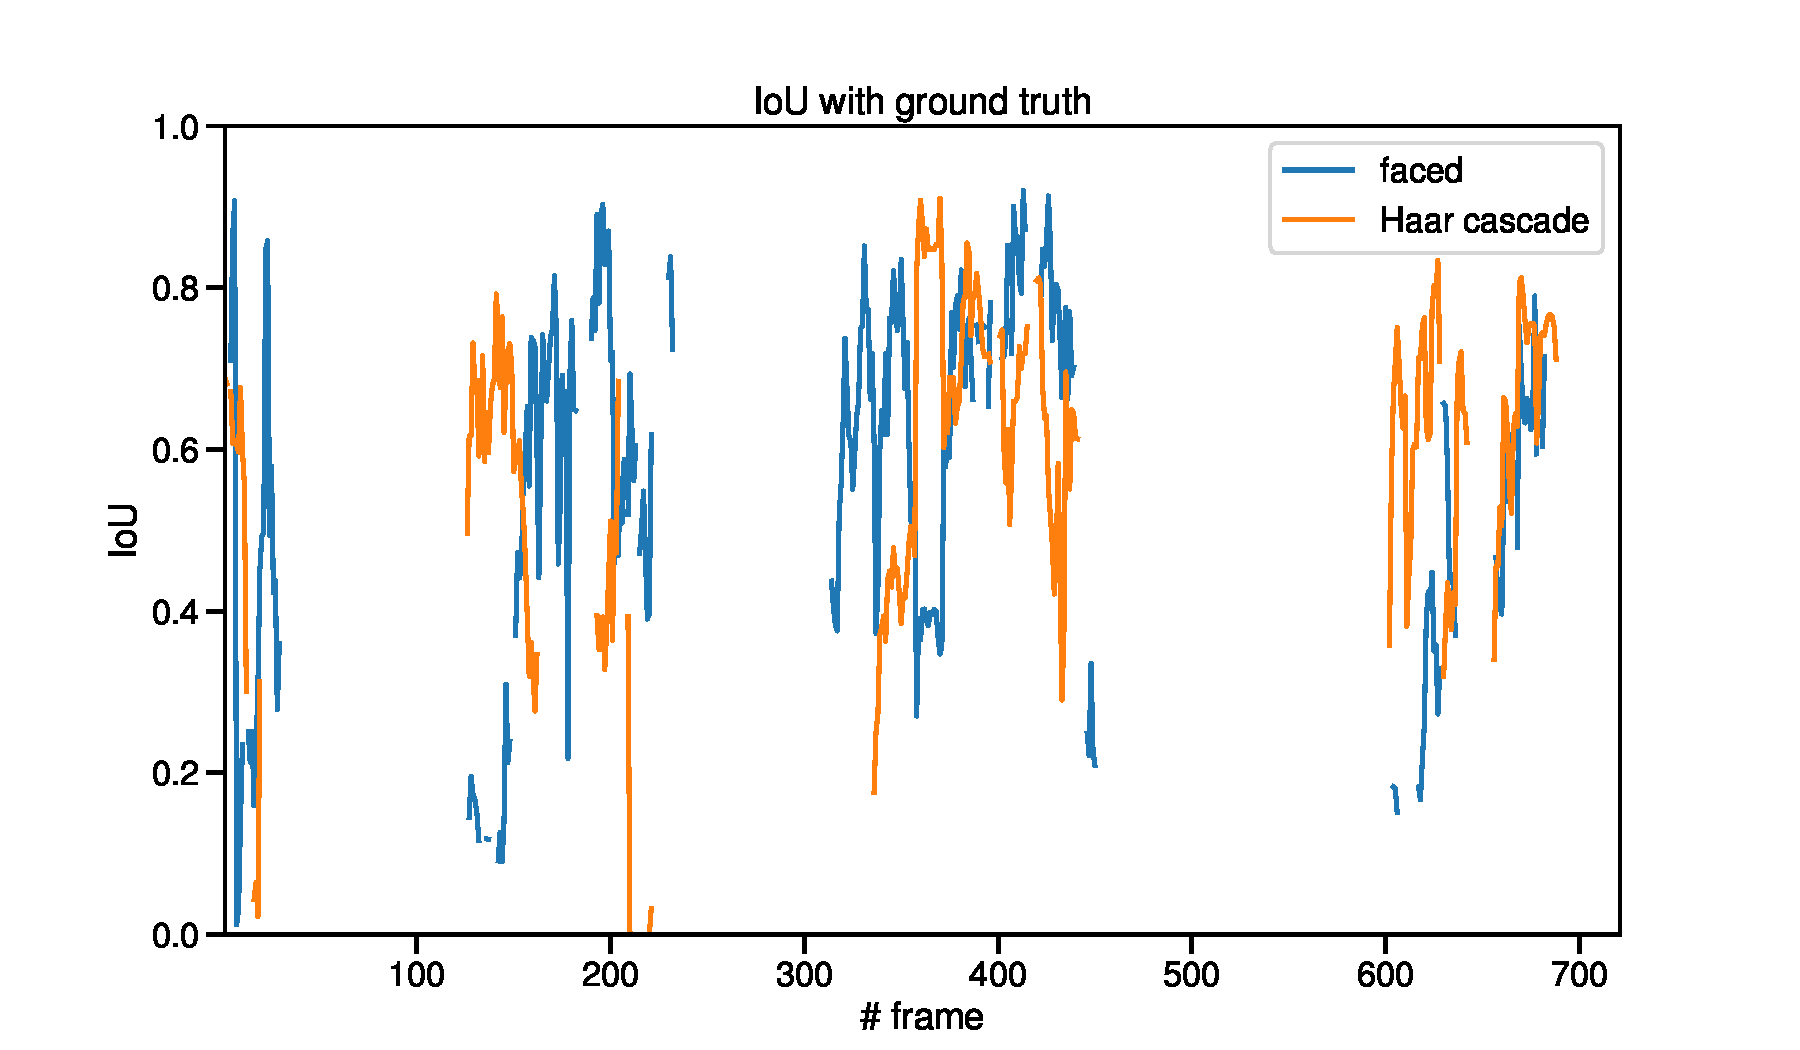
\includegraphics[width=0.8\linewidth]{test2}
	\end{center}

	\begin{table}[h]
		\tiny
		\begin{tabular}{|l|c|c|}
			\hline
			& \textbf{haar}             & \textbf{faced}              \\ \hline
			\textbf{IoU}            & 0.579 $\pm$  0.202 & 0.559 $\pm$  0.221 \\ \hline
			\textbf{Frames with detection} & 248 (34.40\%) & 266 (36.89\%) \\ \hline
		\end{tabular}
	\end{table}
\end{frame}

\begin{frame}
	\frametitle{Face recognition}
	Distance between two faces and the reference face.
	\begin{center}
%		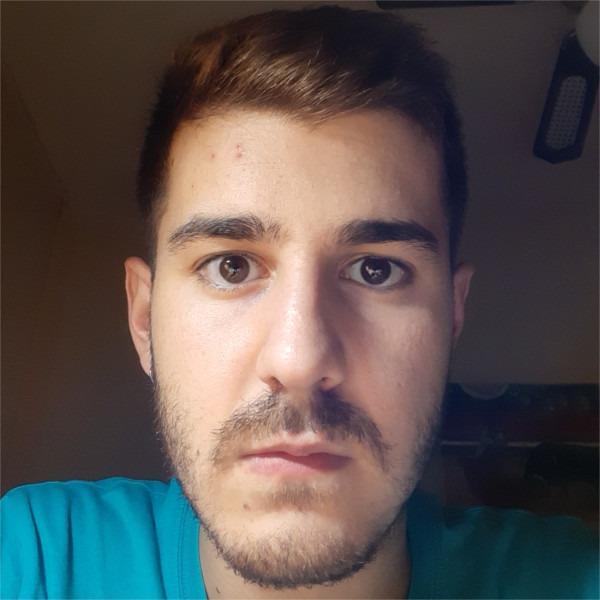
\includegraphics[width=0.2\linewidth]{test4_refface}
		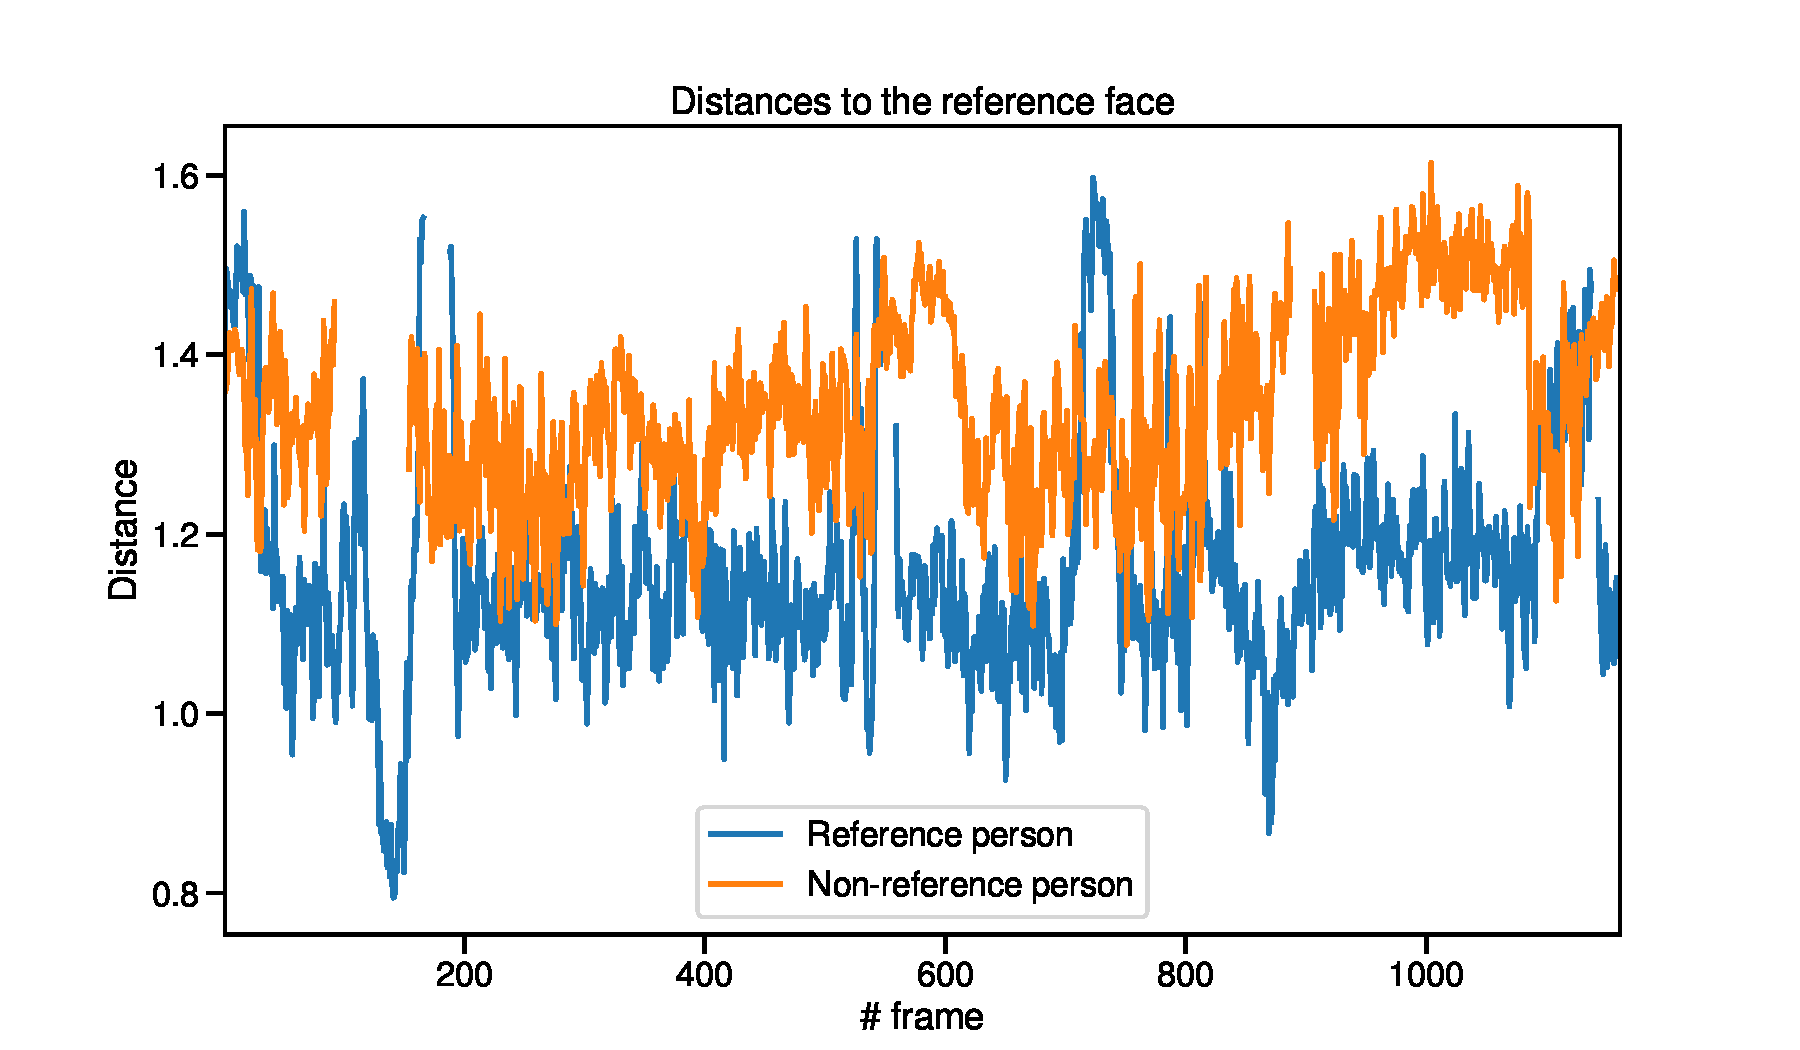
\includegraphics[width=0.85\linewidth]{test4}
	\end{center}

	\begin{table}[h]
		\tiny
		\begin{tabular}{|l|c|c|}
			\hline
			& \textbf{Ref. person} & \textbf{Non-ref. person} \\ \hline
			\textbf{IoU}           & 1.160 $\pm$  0.128 & 1.344 $\pm$  0.102 \\ \hline
		\end{tabular}
	\end{table}	
	
\end{frame}

\begin{frame}
	\frametitle{TensorRT Optimizations}
	Loss in precision and inference time.
	\begin{center}
		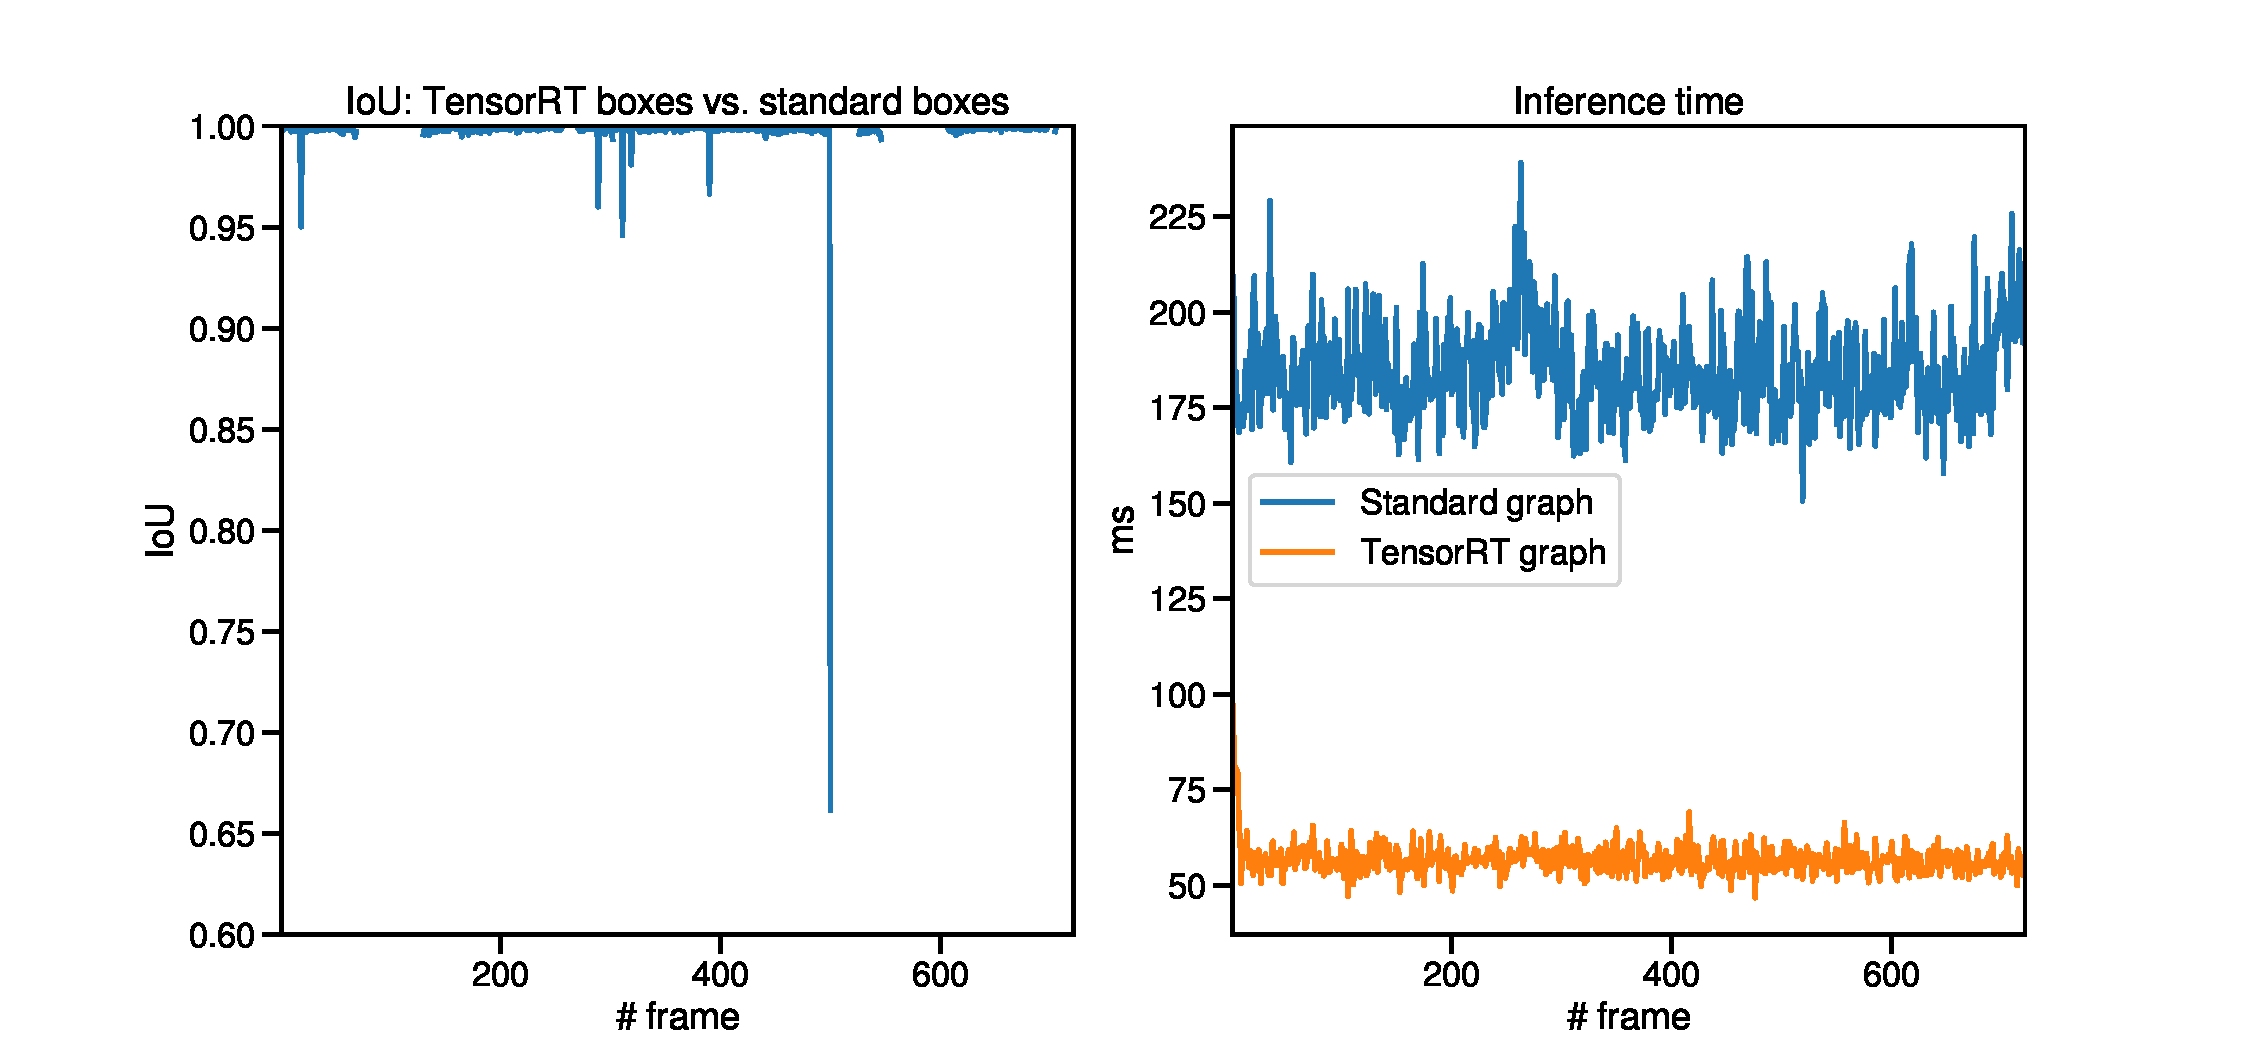
\includegraphics[width=0.9\linewidth]{test3}
	\end{center}
	
	\begin{table}[h]
		\tiny
		\begin{tabular}{|l|c|c|}
			\hline
			& \textbf{Original graph} & \textbf{TensorRT graph} \\ \hline
			\textbf{Inference time (ms)}           & 184.477 $\pm$  11.827 & 56.769 $\pm$  4.148 \\ \hline
			\textbf{IoU with original graph}           & - & 0.997 $\pm$  0.015 \\ \hline
		\end{tabular}
	\end{table}
\end{frame}

\begin{frame}
	\frametitle{Motion tracker}
	Gain in robustness to occlusions using the tracker.
	\begin{center}
		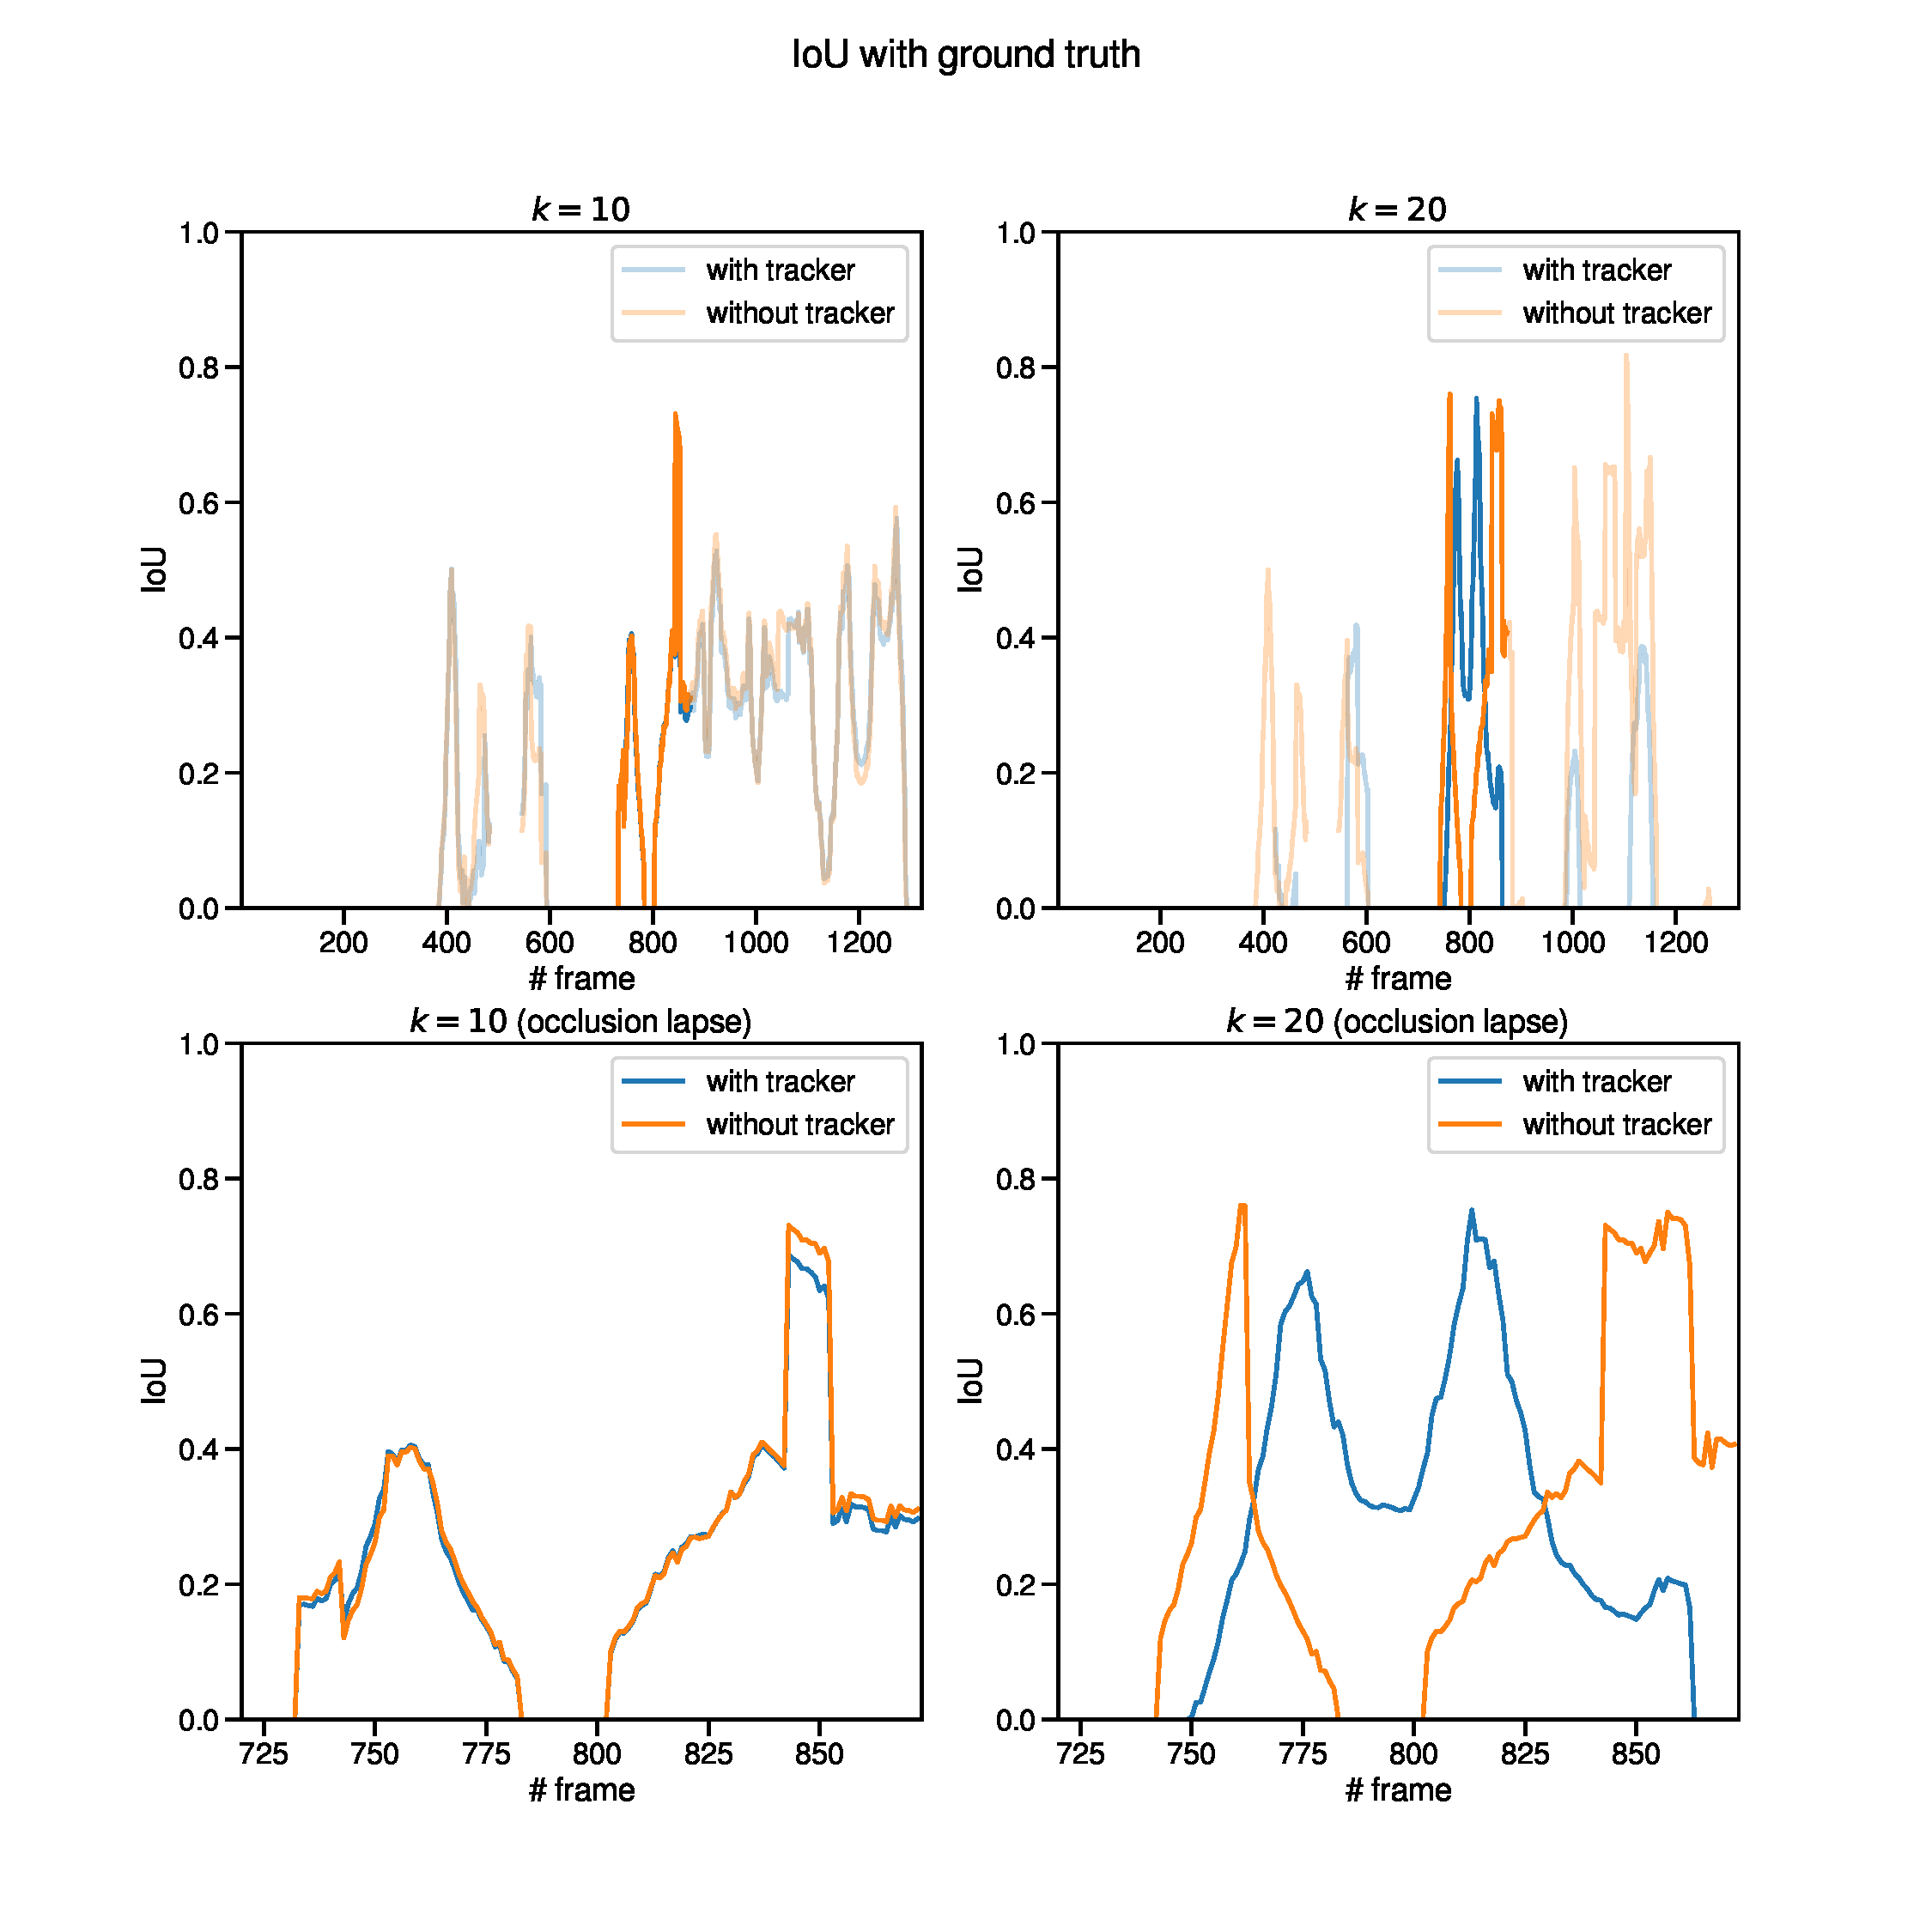
\includegraphics[width=0.75\linewidth]{test5}
	\end{center}
\end{frame}

\begin{frame}
	\frametitle{Full system}
	Following the person.
	\begin{center}
		\href{https://www.youtube.com/watch?v=WZ0riKMwJWA}{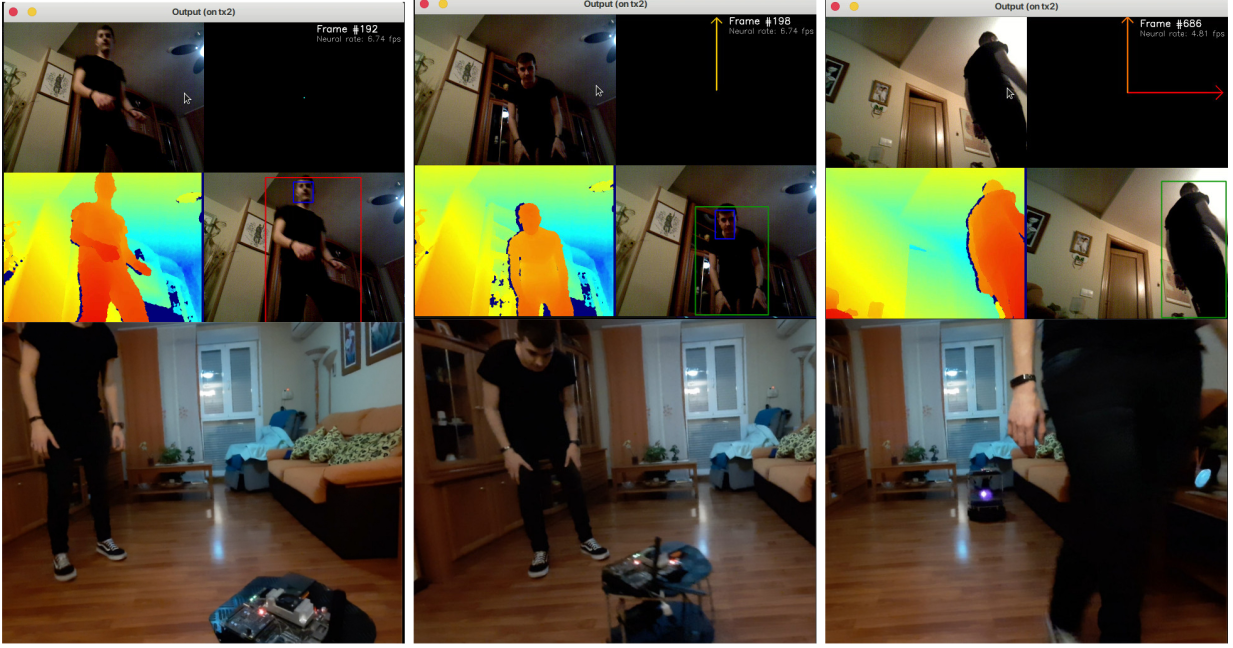
\includegraphics[width=0.75\linewidth]{final_test}}
	\end{center}
\end{frame}

\section{Conclusions}
\begin{frame}
	\frametitle{Conclusions I}
	Accomplishment of the outlined objectives:
	\begin{itemize}
		\item [\faCheck] Real-time following behavior.
		\item [\faCheck] Affordable/educational hardware.\pause
		\item [\faCheck] Robust detection relying on deep learning.\pause
		\item [\faCheck] Enhanced softness using an optical tracker.
	\end{itemize}
\end{frame}
\begin{frame}
	\frametitle{Conclusions II}
	Main drawbacks found:
	\begin{itemize}
		\item [\faClose] Lighting affected by the camera position.\pause
		\item [\faClose] Persons crossing each other may be confounded.\pause
		\item [\faClose] Collisions with obstacles may occur.
	\end{itemize}
\end{frame}

\begin{frame}
	\frametitle{Conclusions III}
	Future lines to address:
	\begin{itemize}
		\item Sensor fusion to enhance the perception.\pause
		\item Probabilistic tracker to model trajectories.\pause
		\item Navigation algorithms for obstacle avoidance.
	\end{itemize}
\end{frame}

\begin{frame}
	\titlepage
\end{frame}

%\begin{frame}
%	\frametitle{Questions}
%\end{frame}
%
%\begin{frame}
%%	\frametitle{Questions}
%	\begin{center}
%		\huge \textbf{Thank you}
%	\end{center}
%\end{frame}

\end{document}